\pdfminorversion=7
%oneside para una impresi\'on simple.
%titlepage define que vamos a tener una portada.
%openany para que los cap\'{\i}tulos empiecen en cualquier p\'agina y no s\'olo las impares.
%final es para compilar a modo normal. Cambiar a draft para que se compile en modo borrador. No se pone final dado que viene por defecto.
\documentclass[a4paper, 12pt, oneside, titlepage, openany]{book}

% Opciones para hyperref. Deben pasarse antes de que cualquier paquete
% (p. ej. pdfcomment) cargue hyperref, para evitar un "Option clash".
\PassOptionsToPackage{plainpages=false,pdfpagelabels}{hyperref}

% Para el seccionado, debe colocarse al principio este package.
\usepackage{titlesec}

% Encoding + cmap (para obtener un mapeo UTF8 adecuado)
\usepackage{cmap}
\usepackage[utf8]{inputenc}
\usepackage[T1]{fontenc} % Para poder copiar y pegar el texto desde un pdf
\usepackage{lmodern}

\usepackage[backend=biber, style=iso-numeric, sorting=nyt, language=spanish]{biblatex}
\DeclareUnicodeCharacter{202F}{~} % Para reemplazar el caracter 202F por un espacio
\bibliography{biblio.bib}
\setcounter{tocdepth}{3}
\setcounter{secnumdepth}{3}
% Esto último es para la cantidad de niveles en el índice

\DeclareFieldFormat{urldate}{\mkbibbrackets{consultado\space#1}}

% Para colores
\usepackage[usenames,dvipsnames]{xcolor}

% Para flotar figuras y tablas
\usepackage{framed}

% Para asegurar que las figuras y tablas queden en la secci\'on correspondiente
\usepackage[section,above,below]{placeins}

% Para microtipograf\'{\i}a
\usepackage{microtype}

% Permite tama\~no de fuentes arbitrarios
\usepackage{anyfontsize}

% Itemize
\usepackage{enumitem}
\newlist{Properties}{enumerate}{2}
\setlist[Properties]{label=Propiedad \arabic*.,itemindent=*}
\renewcommand{\labelitemii}{\textasteriskcentered}
\renewcommand{\labelitemiii}{-}

\usepackage{lastpage} % Para poder contar las p\'aginas, habilita el \pageref command.
\usepackage{titleps} % Para la tabla de contenidos
\usepackage{textcase}
\usepackage{pdfpages}

% \parbox[b] es para poner texto sobre el bottom
\newpagestyle{ruled}{
	\sethead{
\includegraphics[width=3.7cm]{./images/UADE_LARGE}}
			{\parbox[b]{0.43\textwidth}{\raggedright\MakeUppercase{DePaso --- Logística urbana colaborativa}}}
			{
				\raisebox{1.5ex}{%
					\parbox[b]{0.26\textwidth}{\raggedleft
					\begin{tabular}{r}
						Toffoletto, Martina O. \\
						Basaez, Candela P.
					\end{tabular}
					}
				}
			}\headrule{}
	\setfoot[][][P\'agina \thepage\ de~\pageref*{LastPage}]{}{}{P\'agina \thepage\ de~\pageref*{LastPage}}\footrule{}
	}
\pagestyle{ruled}
% Cambiar el color de la linea divisora:
% \renewcommand\makeheadrule{\color{cyan}\rule[-.3\baselineskip]{\linewidth}{0.4pt}}
% \renewcommand\makefootrule{\color{cyan}\rule[\baselineskip]{\linewidth}{0.4pt}}

% Para que la primera página de cada capítulo no sea tratada como especial
\makeatletter
\let\ps@plain\ps@ruled
\makeatother

% M\'argenes
\usepackage{vmargin}
%\setmarginsrb{leftmargin}{topmargin}{rightmargin}{bottommargin}%
%         {headheight}{headsep}{footheight}{footskip}           %
%Lo ideal ser\'{\i}a lo siguiente
%\setmarginsrb{2.7cm}{4cm}{2.3cm}{2.5cm}{2cm}{0.5cm}{2cm}{0.5cm}
%Pero estos valores se suman, por lo que en realidad ir\'{\i}a asi:
% headheight debe alcanzar para el logo UADE del encabezado (~1.3cm); se
% compensa restando de headsep para que el bloque de texto no se desplace.
\setmarginsrb{2.7cm}{2cm}{2.3cm}{1.5cm}{1.31cm}{0.69cm}{0cm}{1cm}
% M\'argenes, pero otra opci\'on mas acotada
% \usepackage[top=4cm,bottom=2.5cm,left=2.7cm,right=2.3cm]{geometry}

% Seccionado. El par\'ametro left incrementa el margen, lo setteo en 0.
%\titlespacing*{<command>}{<left>}{<before-sep>}{<after-sep>}
% \titlespacing{\section}{0pt}{12pt}{6pt}
%\titlespacing{\subsection}{0pt}{*0}{*0}
%\titlespacing{\subsubsection}{0pt}{*0}{*0}

%Tama\~no de letra de cap\'{\i}tulo y secciones
%\newcommand{\chapfnt}{\fontsize{16}{19}}
%\newcommand{\secfnt}{\fontsize{14}{17}}
%\newcommand{\ssecfnt}{\fontsize{12}{14}}
%\titleformat{\chapter}[display]
%{\normalfont\chapfnt\bfseries}{\chaptertitlename\ \thechapter}{20pt}{\chapfnt}
%\titleformat{\section}
%{\normalfont\secfnt\bfseries}{\thesection}{1em}{}
%\titleformat{\subsection}
%{\normalfont\ssecfnt\bfseries}{\thesubsection}{1em}{}

% Se pide numeraci\'on de tablas en n\'umeros romanos
\renewcommand{\thetable}{\thechapter.\Roman{table}}

%Espaciado antes y despu\'es de una figura respecto del texto
\setlength{\textfloatsep}{5pt}

% Para notas
\usepackage{todonotes}
\setlength{\marginparwidth}{2cm} % El margen es muy estrecho. Esto es solo para solucionar un warning
\newcommand{\Nico}[1]{\todo[color=green!30,inline]{\textbf{Nico:} #1}}
\newcommand{\Fermat}[1]{\todo[color=green!30]{\textbf{Fermat:} #1}}

%Espaciado entre referencias en la bibliograf\'{\i}a
\usepackage{etoolbox}
\patchcmd{\thebibliography}
  {\settowidth}
  {\setlength{\itemsep}{6pt}\settowidth}
  {}{}
\apptocmd{\thebibliography}
  {\small}
  {}{}

\usepackage{pdfcomment}
\usepackage{pgfgantt}
\usepackage{booktabs}
\usepackage{graphicx}
\usepackage{float}

% Marcado de contenido nuevo (entrega 50%) para revisión del tutor.
% Envolver los bloques nuevos con \nuevo{...} o {\color{nuevo} ...}.
% El documento se entrega en NEGRO: el color queda en 0,0,0 y los marcados
% \nuevo{...} no se ven. Para volver a resaltar lo nuevo mientras se trabaja,
% poner {0,0,205}. Las diferencias contra main se ven con ./make-diff.sh.
\definecolor{nuevo}{RGB}{0,0,0}
\newcommand{\nuevo}[1]{{\color{nuevo}#1}}

% Marcador de posición para material todavía no incorporado (fotos de user
% personas, mockups, capturas de la demo). Dibuja un recuadro punteado del
% tamaño indicado con una leyenda adentro.
%   Uso: \marcador[ancho]{alto}{leyenda}
%   Al incorporar el material real, se reemplaza la línea completa por:
%   \includegraphics[width=...]{figures/nombre-del-archivo}
\newcommand{\marcador}[3][0.45\textwidth]{%
    \begin{tikzpicture}
        \node[draw=black!45, dashed, thick, rounded corners=3pt, fill=black!4,
              minimum width=#1, minimum height=#2, align=center, inner sep=4pt,
              font=\footnotesize\itshape, text=black!55] {#3};
    \end{tikzpicture}%
}

% TikZ para los diagramas del dise\~no (C4, casos de uso, secuencia, despliegue, DER)
\usepackage{tikz}
\usetikzlibrary{positioning, arrows.meta, shapes.geometric, shapes.multipart, fit, backgrounds, calc}
\tikzset{
    c4person/.style={draw, rounded corners=2pt, fill=RoyalBlue!15, minimum width=2.3cm, minimum height=1cm, align=center, font=\footnotesize},
    c4system/.style={draw, rounded corners=7pt, fill=ForestGreen!18, minimum width=3cm, minimum height=1.3cm, align=center, font=\footnotesize},
    c4container/.style={draw, rounded corners=3pt, fill=RoyalBlue!10, minimum width=2.9cm, minimum height=1.2cm, align=center, font=\footnotesize},
    c4ext/.style={draw, rounded corners=2pt, fill=black!8, minimum width=2.5cm, minimum height=1cm, align=center, font=\footnotesize},
    c4db/.style={draw, cylinder, shape border rotate=90, aspect=0.25, fill=black!8, minimum width=2.3cm, minimum height=1.3cm, align=center, font=\footnotesize, inner sep=3pt},
    c4arrow/.style={-{Stealth[length=2mm]}, thick},
    c4lbl/.style={font=\scriptsize, fill=white, inner sep=1pt, midway},
    ucase/.style={draw, ellipse, align=center, font=\scriptsize, fill=Goldenrod!20, minimum width=3.1cm, minimum height=0.9cm, inner sep=1pt},
    boundary/.style={draw, thick, rounded corners=4pt},
    entity/.style={draw, rectangle split, rectangle split parts=2, fill=RoyalBlue!8, font=\scriptsize, align=left, minimum width=2.6cm},
}
% Actor UML (figura de palotes) como pic reutilizable
\tikzset{
    actor/.pic={
        \draw[thick] (0,0) circle (2.4mm);
        \draw[thick] (0,-2.4mm) -- (0,-1cm);
        \draw[thick] (-4.5mm,-6mm) -- (4.5mm,-6mm);
        \draw[thick] (0,-1cm) -- (-3.5mm,-1.6cm);
        \draw[thick] (0,-1cm) -- (3.5mm,-1.6cm);
    }
}
\usepackage[spanish,es-nodecimaldot]{babel}
\usepackage{csquotes}
\addto\captionsspanish{
	\renewcommand{\contentsname}{\'Indice}
	\renewcommand{\listfigurename}{Lista de Figuras}
	\renewcommand{\listtablename}{Lista de Tablas}
	\renewcommand{\tablename}{TABLA}
}

% Para que el primer parrafo de un cap\'{\i}tulo tenga identado.
\usepackage{indentfirst}
\setlength{\parindent}{36pt} %Tama\~no de la identaci\'on.

% Para tablas complejas
\usepackage{multicol,multirow}
\usepackage{array,longtable}

% Times New Roman para texto y matemáticas. Debe ir antes de los paquetes AMS.
\usepackage{mathptmx}

\usepackage{amsmath,amsfonts,amssymb,amsthm}

\allowdisplaybreaks{} % Para que el align permita dividir entre p\'aginas si lo llega a necesitar.

\usepackage{cancel}

\newenvironment{example}[1][Ejemplo]{\begin{trivlist}
	\item[\hspace{\labelsep} {\itshape{} #1}]}{\end{trivlist}}

\newenvironment{examples}[1][Ejemplos]{\begin{trivlist}
	\item[\hspace{\labelsep} {\itshape{} #1}]}{\end{trivlist}}

\newenvironment{EstadoDelArte}
    {\small\begin{center}
    \bfseries{EstadoDelArte} \end{center}}

\newenvironment{Enfoque metodologico}
    {\small\begin{center}
    \bfseries{Enfoque metodologico} \end{center}}

\newenvironment{Cronograma}
    {\small\begin{center}
    \bfseries{Cronograma} \end{center}}

\input{config/symbols}

\usepackage[normalem]{ulem}

\usepackage{setspace}
\onehalfspacing

% En UADE no existe la noción de capítulo en la tesis, por más que en LaTeX sí lo tratemos como tal.
% Además nos piden que el tamaño de letra de lo que para nosotros es una sección, subsección y demás, sean del mismo tamaño.
\titleformat{\chapter}
  {\bfseries\fontsize{14pt}{14pt}\selectfont}
  {\thechapter}{1em}{}
\titlespacing*{\chapter}{0pt}{12pt}{6pt}

\titleformat{\section}
  {\bfseries\fontsize{14pt}{14pt}\selectfont}
  {\thesection}{1em}{}
\titlespacing*{\section}{0pt}{12pt}{6pt}

\titleformat{\subsection}
  {\bfseries\fontsize{14pt}{14pt}\selectfont}
  {\thesubsection}{1em}{}
\titlespacing*{\subsection}{0pt}{12pt}{6pt}

\titleformat{\subsubsection}
  {\bfseries\fontsize{14pt}{14pt}\selectfont}
  {\thesubsubsection}{1em}{}
\titlespacing*{\subsubsection}{0pt}{12pt}{6pt}

% -> Acá se empieza a modificar el tamaño de los títulos autogenerados, como los de las listas de figuras y tablas
\usepackage{tocloft}
\cftsetindents{table}{0em}{4em}

\renewcommand{\cfttoctitlefont}{\bfseries\fontsize{14pt}{16pt}\selectfont}
\setlength{\cftbeforetoctitleskip}{12pt}
\setlength{\cftaftertoctitleskip}{6pt}

% Fuente del título (14pt, negrita)
\renewcommand{\cftloftitlefont}{\bfseries\fontsize{14pt}{16pt}\selectfont}
\renewcommand{\cftlottitlefont}{\bfseries\fontsize{14pt}{16pt}\selectfont}

% Espaciado antes y después del título
\setlength{\cftbeforeloftitleskip}{12pt}
\setlength{\cftafterloftitleskip}{6pt}
\setlength{\cftbeforelottitleskip}{12pt}
\setlength{\cftafterlottitleskip}{6pt}


% IMPORTANTE: En la entrega final de UADE se debe dejar sin color. Usar el bloque comentado a continuación y comentar el bloque activo.
\usepackage{hyperref}
\hypersetup{
    colorlinks,
    linkcolor=black,
    citecolor=red
}
\renewcommand{\theHtable}{\thechapter.\Roman{table}}
\renewcommand{\theHfigure}{\thechapter.\arabic{figure}}
% Para la entrega final:
%\usepackage[hidelinks]{hyperref}
%\hypersetup{
%    colorlinks=false,
%    pdfborder={0 0 0},
%    linktoc=none
%}

\DefineBibliographyStrings{spanish}{
  online   = {En línea},
  urlfrom  = {Disponible en:},
  andothers = {\mkbibemph{et\addabbrvspace al\adddot}}
}

\begin{document}
\hypersetup{pageanchor=false}
\clearpage
\thispagestyle{empty}

\includepdf[
  pages=1,
  scale=1.01, %1.17
  offset=25mm -25mm,
  pagecommand={\thispagestyle{empty}},
  noautoscale,
  trim=0 0 0 0,
  clip
]{cover/caratula_DePaso.pdf}
\clearpage
	\begin{titlepage}
    \centering

    {\textbf{\fontsize{18}{20}\selectfont PROYECTO FINAL DE INGENIERÍA} \par}
    \vspace{1.5cm}

    {\textbf{\fontsize{16}{18}\selectfont DePaso} \par}
    \vspace{0.5cm}

    {\textbf{\fontsize{14}{16}\selectfont Toffoletto, Martina Ornella --- LU 1139965} \par}
    {\fontsize{14}{16}\selectfont Ingeniería en Informática \par}
    \vspace{1cm}

    {\textbf{\fontsize{14}{16}\selectfont Basaez, Candela Pilar --- LU 1134260} \par}
    {\fontsize{14}{16}\selectfont Ingeniería en Informática \par}
    \vspace{1.5cm}

    {\fontsize{14}{16}\selectfont Tutor: \par}
    {\textbf{\fontsize{14}{16}\selectfont Dos Santos, Maximiliano Luis,
		\\ (UADE) Universidad Argentina de la Empresa Lima 757, Cdad. Autónoma de Buenos Aires, Argentina.
			} \par}
    \vspace{3cm}

	{\textbf{\fontsize{14}{16}\selectfont \the\year} \par}
    % {\textbf{\fontsize{14}{16}\selectfont 2025} \par} % se puede hardcodear
	% {\textbf{\fontsize{14}{16}\selectfont \today} \par} % fecha completa si es la entrega final
    \vspace{2cm}

    
\includegraphics[width=0.30\textwidth]{./images/UADE}\par \vspace{1cm}
    {\textbf{\fontsize{14}{16}\selectfont UNIVERSIDAD ARGENTINA DE LA EMPRESA} \par}
    {\fontsize{14}{16}\selectfont FACULTAD DE INGENIERÍA Y CIENCIAS EXACTAS \par}
\end{titlepage}
	\newpage
\hypersetup{pageanchor=true}
	\tableofcontents
	\chapter{Introducción}

DePaso es una plataforma digital de logística urbana colaborativa orientada a PyMEs, comercios y clientes particulares del Área Metropolitana de Buenos Aires (AMBA). Su propósito es facilitar la gestión integral de envíos urbanos mediante una solución que permita solicitar, asignar, monitorear y completar entregas de manera eficiente, incorporando además herramientas para estimar el impacto ambiental asociado a cada operación.

A diferencia de las plataformas de envíos bajo demanda actualmente disponibles, que se basan principalmente en transportistas dedicados, DePaso propone un modelo híbrido que combina transporte exclusivo con transporte colaborativo. Este último aprovecha trayectos que los transportistas ya realizan por motivos propios, permitiendo utilizar capacidad disponible en desplazamientos existentes y reduciendo viajes adicionales mediante mecanismos de asignación que minimizan los desvíos.

La propuesta surge ante una serie de problemáticas presentes en la logística urbana actual:

\begin{itemize}[leftmargin=2em]
    \item Costos logísticos elevados para PyMEs y comercios que no cuentan con flota propia.
    \item Existencia de vehículos que realizan trayectos con capacidad disponible sin ser aprovechada.
    \item Ineficiencias en la distribución de última milla dentro de entornos urbanos densamente poblados.
    \item Emisiones de CO\textsubscript{2} asociadas a viajes dedicados que podrían evitarse mediante esquemas colaborativos.
    \item Escasas oportunidades para que personas que realizan desplazamientos cotidianos obtengan ingresos adicionales aprovechando sus recorridos habituales.
\end{itemize}

{\color{nuevo}La magnitud de estas problemáticas se refleja en datos del sector. La entrega de última milla concentra una fracción desproporcionada del costo logístico total y constituye el tramo más ineficiente de la cadena de distribución \parencite{YangEtAl2022}. En Argentina esa presión se intensifica: el Índice de Costos Logísticos elaborado por la Cámara Empresaria de Operadores Logísticos, homologado por la Universidad Tecnológica Nacional, acumuló un incremento del 22,2~\% en el primer semestre de 2026, muy por encima del 14~\% registrado en el mismo período del año anterior \parencite{CEDOL2025}. Esta ineficiencia tiende a agravarse: de mantenerse las tendencias actuales, se proyecta que para 2030 la demanda de entregas urbanas crezca un 78~\%, con un aumento del 36~\% en la cantidad de vehículos de reparto, del 32~\% en las emisiones de CO\textsubscript{2} y del 21~\% en la congestión de las principales ciudades \parencite{WEF2020}. En Argentina, el transporte explica cerca del 14~\% de las emisiones totales de gases de efecto invernadero del país, siendo la segunda fuente de emisiones dentro del sector energético \parencite{InventarioGEI2024}. En el plano local, un relevamiento de la Organización Internacional del Trabajo sobre trabajadores de plataformas de reparto en la Argentina encontró que el 95~\% de quienes habían ingresado recientemente lo hizo ante la dificultad de conseguir otro empleo; hacia fines de 2018, solo tres de las principales aplicaciones de reparto (Glovo, PedidosYa y Rappi) sumaban en conjunto más de 7.100 repartidores independientes registrados, la amplia mayoría bajo la figura de monotributista y sin relación de dependencia \parencite{OIT2020}.}

Frente a este escenario, DePaso busca articular una solución que aproveche la capacidad ociosa existente en los desplazamientos urbanos, al tiempo que ofrece alternativas de envío dedicado para los casos que así lo requieran. El proyecto se circunscribe a dicha área metropolitana y tiene como horizonte temporal el desarrollo de un prototipo funcional para finales de 2026. Esta combinación se traduce en un conjunto de modalidades de servicio que estructuran la operación de la plataforma y que se describen a continuación.

% ─────────────────────────────────────────────────────────────────────────────
\section{Modalidades de envío}

DePaso organiza sus servicios a partir de dos dimensiones: la forma en que se inicia la operación y el tipo de trayecto realizado por el transportista. La combinación de ambas da lugar a cuatro modalidades de servicio:

\begin{itemize}[leftmargin=2em]
    \item \textbf{Dedicado por demanda}: el remitente solicita un envío y el sistema identifica transportistas disponibles cercanos al punto de origen.
    
    \item \textbf{Dedicado por espacio}: el transportista informa disponibilidad en una zona y franja horaria determinadas, permitiendo la asignación de pedidos compatibles con la capacidad de su vehículo.
    
    \item \textbf{Colaborativo por demanda}: el remitente solicita un envío con cierta flexibilidad temporal y el sistema busca trayectos existentes compatibles con el recorrido requerido, procurando minimizar el desvío adicional.
    
    \item \textbf{Colaborativo por espacio}: el transportista registra trayectos habituales recurrentes y recibe sugerencias de envíos compatibles con dichos recorridos.
\end{itemize}

Para la operación del sistema se contemplan cuatro categorías generales de carga: paquetes pequeños y documentos, cargas medianas, cargas grandes o voluminosas y mudanzas o fletes. Las restricciones según el tipo de movilidad disponible se presentan en la Tabla~\ref{tab:restricciones}.
\begin{table}[H]
    \caption{Restricciones de carga por tipo de movilidad}
    \label{tab:restricciones}
    \centering
    \small
    \begin{tabular}{lccccc}
        \toprule
        \textbf{Categoría} & \textbf{Peatón/Bici} & \textbf{Moto} & \textbf{Auto} & \textbf{Camioneta} & \textbf{Camión} \\
        \midrule
        Pequeños / documentos & Sí\textsuperscript{*} & Sí & Sí & Sí & Sí \\
        Medianos              & No & Sí & Sí & Sí & Sí \\
        Grandes / voluminosos & No & No & Sí & Sí & Sí \\
        Mudanzas / fletes     & No & No & No & Sí & Sí \\
        \bottomrule
        \multicolumn{6}{l}{\textsuperscript{*} Solo trayectos cortos ($<$ 5 km).}
    \end{tabular}
\end{table}

Las mudanzas y fletes se asignan siempre en modalidad dedicada; nunca colaborativa.

% ─────────────────────────────────────────────────────────────────────────────
\vspace{1em}
\section{Objetivos}

\subsection{Objetivo general}

Desarrollar, para fines de 2026, un prototipo funcional de plataforma digital de logística urbana colaborativa para el AMBA que permita gestionar el ciclo completo de los envíos mediante mecanismos inteligentes de clasificación y asignación, aprovechando la capacidad disponible en los desplazamientos de los transportistas.

\subsection{Objetivos específicos}

{\color{nuevo}
\begin{itemize}[leftmargin=2em]
    \item Desarrollar e implementar un sistema de visión computacional capaz de clasificar automáticamente las cargas en las cuatro categorías volumétricas definidas a partir de imágenes, alcanzando una exactitud (\emph{accuracy}) sobre el conjunto de prueba de al menos el 60\%, valor que supera ampliamente la línea base aleatoria del 25\% correspondiente a cuatro categorías.

    \item Implementar un mecanismo de asignación inteligente que evalúe la compatibilidad entre pedidos y transportistas considerando características de la carga, trayectorias, ventanas horarias y reputación, y que restrinja el desvío del transportista colaborativo a un máximo del 15\% del trayecto original mediante un filtro duro, devolviendo un ranking de candidatos con su puntaje desglosado y explicable.

    \item Incorporar un modelo híbrido de operación que contemple tanto envíos dedicados como colaborativos, cubriendo las cuatro categorías de carga y los distintos tipos de movilidad definidos.

    \item Desarrollar un mecanismo de estimación del impacto ambiental que calcule el ahorro de CO\textsubscript{2} del 100\% de los envíos colaborativos completados respecto de un escenario equivalente de transporte dedicado, a partir de factores de emisión estandarizados por tipo de vehículo, verificando el cálculo mediante pruebas automatizadas con coordenadas reales del AMBA.

    \item Diseñar e implementar una plataforma digital con una arquitectura modular preparada para escalar, que integre los distintos componentes funcionales necesarios para la gestión de envíos urbanos, con una cobertura geográfica objetivo del AMBA y con pruebas automatizadas sobre la totalidad de los módulos críticos, incluidos los flujos de integración de punta a punta.
\end{itemize}
}

% ─────────────────────────────────────────────────────────────────────────────
\vspace{1em}
\section{Alcance}

El proyecto comprende el diseño y desarrollo de un prototipo funcional de plataforma digital para la gestión logística de envíos dentro del AMBA.

\subsection{Características del prototipo funcional}

El sistema incluirá:

\begin{itemize}[leftmargin=2em]
    \item Registro y autenticación de clientes y transportistas con distintos medios de movilidad.
    
    \item Creación, asignación y seguimiento de pedidos en las diferentes modalidades de servicio definidas.
    
    \item Clasificación automática de cargas mediante inteligencia artificial, con posibilidad de ingreso manual alternativo.
    
    \item Asignación inteligente basada en trayectorias geográficas compatibles.
    
    \item Gestión de capacidad disponible de los vehículos.
    
    \item Estimación del ahorro de CO\textsubscript{2} asociado a envíos colaborativos.
    
    \item Herramientas básicas de monitoreo operativo para administradores.
\end{itemize}

\vspace{1em}
\subsection{Limitaciones y exclusiones}

El alcance se restringe geográficamente a operaciones dentro del AMBA, excluyendo envíos interprovinciales e internacionales. El clasificador de carga estará acotado a las categorías volumétricas definidas y al dataset de entrenamiento, ofreciendo el ingreso manual como alternativa cuando el objeto no sea reconocido con confianza suficiente. La pasarela de pagos se simulará en el prototipo, dejando su integración productiva como trabajo posterior. El mecanismo de cobertura ante daños se abordará a nivel de diseño y definición de responsabilidades, quedando la integración con compañías aseguradoras fuera del alcance del prototipo.

\subsection{Estructura del documento}

El presente documento se organiza de la siguiente manera: el Capítulo~1 introduce el problema, las modalidades de servicio, los objetivos y el alcance del proyecto; el Capítulo~2 presenta los antecedentes, compuestos por el marco teórico, el estado del arte y {\color{nuevo}el análisis competitivo}; el Capítulo~3 describe la propuesta y la investigación de usuarios realizada; {\color{nuevo}el Capítulo~4 detalla el análisis de requerimientos, con los requerimientos funcionales y no funcionales y los casos de uso; el Capítulo~5 desarrolla la metodología de desarrollo, la arquitectura y las tecnologías, el modelo de datos y la validación del sistema; y el Capítulo~6} expone la conclusión parcial y el trabajo futuro. Completan el documento la bibliografía y los anexos, que incluyen el cronograma de actividades{\color{nuevo}, la transcripción de los resultados de la encuesta y la transcripción de las entrevistas semiestructuradas}.
	\chapter{Antecedentes}

% ═════════════════════════════════════════════════════════════════════════════
\section{Marco teórico}

El desarrollo de una plataforma de logística urbana colaborativa requiere integrar conceptos provenientes de distintas áreas: logística de última milla, modelos de transporte colaborativo, mecanismos de asignación entre oferta y demanda e inteligencia artificial.

El objetivo de este marco teórico es presentar los conceptos que fundamentan las principales decisiones de diseño adoptadas en DePaso. En primer lugar se analizan los modelos de crowdsourced delivery y las flotas híbridas como alternativa a los sistemas tradicionales de reparto. Luego se estudian los distintos perfiles de transportistas y los mecanismos de matching utilizados para asignar envíos de forma eficiente. Finalmente se abordan las técnicas de inteligencia artificial aplicadas a la clasificación automática de cargas y se declara el plan de datos que sustentará el entrenamiento de ese clasificador.

Estos conceptos constituyen la base teórica sobre la cual se construye la propuesta desarrollada en este trabajo.
% ─────────────────────────────────────────────────────────────────────────────
\subsection{Crowdsourced delivery y logística de última milla}

El \emph{crowdsourced delivery} (CSD) es un modelo logístico que delega la entrega de última milla a personas no profesionales que integran pedidos en sus propios desplazamientos, a cambio de una compensación económica, en lugar de recurrir a una flota dedicada. A diferencia de los sistemas tradicionales de reparto, no genera viajes nuevos: aprovecha los desplazamientos que ya existen en la ciudad.

Este modelo surge como respuesta a una ineficiencia estructural de la logística urbana. La entrega al destinatario final concentra una fracción desproporcionada del costo logístico total y genera congestión vehicular y emisiones en ciudades densas \parencite{YangEtAl2022}. En el AMBA, esa ineficiencia se agrava: una PyME o un particular que necesita enviar algo enfrenta pocas opciones reales, pagar una tarifa alta por un flete dedicado, resignarse a los tiempos de un \emph{courier} masivo pensado para \emph{e-commerce} de gran volumen, o directamente no enviarlo. Al mismo tiempo, hay vehículos circulando por la ciudad con espacio disponible todos los días y personas que necesitan mandar cosas, y los dos grupos rara vez se cruzan.

Yang \textit{et al.}\ formalizan la lógica del CSD distinguiendo entre vehículos dedicados (DVs), que viajan exclusivamente para hacer entregas, y vehículos personales compartidos (SPVs), cuyos conductores integran pedidos en viajes que ya tenían planificados \parencite{YangEtAl2022}. La diferencia no es solo operativa: define dos modelos logísticos con costos, emisiones y dinámicas de participación completamente distintos, y es la base sobre la que se construye cualquier comparación rigurosa entre el modelo colaborativo y el dedicado.

DePaso se apoya en ese modelo para dar respuesta al problema logístico del AMBA. No opera flota propia ni subcontrata \emph{couriers}: conecta a remitentes con personas que ya se desplazan por la ciudad. Los subtemas que siguen desarrollan los conceptos que hacen viable esa conexión: qué tipo de conductor la sostiene, cómo se asignan pedidos a rutas preexistentes y qué rol cumple la inteligencia artificial en el proceso.

% ─────────────────────────────────────────────────────────────────────────────
\subsection{Flotas híbridas: ventajas del modelo y el problema del desvío}

El resultado central de Yang et al.\ establece que los SPVs reducen el costo unitario de entrega respecto a los DVs, pero que esa ventaja puede revertirse cuando el conductor se aleja demasiado de su ruta habitual para retirar o entregar un paquete: si el desvío supera cierto umbral, los kilómetros adicionales recorridos eliminan el beneficio ambiental e incluso pueden incrementar las emisiones por encima del escenario dedicado que se supone reemplazar \parencite{YangEtAl2022}. Este hallazgo no es un detalle técnico: define una restricción estructural para cualquier plataforma que combine DVs y SPVs.

La implicación de diseño es que el desvío de los conductores debe ser una variable explícita del algoritmo de asignación, no un parámetro secundario. Una plataforma que asigna pedidos sin acotar el desvío puede estar generando más emisiones que el modelo dedicado que dice reemplazar, sin que ni el remitente ni el transportista lo sepan. Yang et al.\ identifican además que este efecto escala con el tamaño del sistema, lo que vuelve al problema especialmente relevante para una plataforma con vocación de alcance masivo.

DePaso traduce este resultado en una restricción de diseño explícita: la modalidad colaborativa solo asigna pedidos cuando el desvío del transportista se mantiene por debajo de un umbral calculado sobre rutas geoespaciales reales. El valor concreto de ese umbral y el mecanismo de cálculo se especifican en etapas posteriores del desarrollo.

% ─────────────────────────────────────────────────────────────────────────────
\subsection{Perfiles de conductores: gig-workers y conductores ocasionales}

La literatura en CSD distingue dos perfiles de conductores según su relación con la plataforma. Luy et al.\ los formalizan en el contexto de flotas híbridas \parencite{LuyEtAl2023}:

\begin{itemize}[leftmargin=2em]
    \item \textbf{Gig-workers (GW)}: conductores con disponibilidad continua que aceptan cualquier pedido dentro de su zona operativa, independientemente de si tienen un destino previo. Maximizan la previsibilidad de la oferta, pero requieren una remuneración constante que se traslada al costo del servicio.
    \item \textbf{Conductores ocasionales (OD, \emph{Occasional Drivers})}: personas que solo participan cuando un pedido coincide con un desplazamiento que ya tienen planificado, como ir al trabajo, a otro barrio o al médico. No son repartidores; son viajeros habituales que ofrecen su capacidad ociosa de forma intermitente.
\end{itemize}

La diferencia entre ambos perfiles no es de grado sino de naturaleza: un OD no es un GW con menos disponibilidad. Su lógica de participación es distinta, su motivación es distinta y, como demuestran Luy et al., el valor que generan depende de que la plataforma reconozca esa diferencia en su diseño. Los autores señalan que la mayoría de las plataformas existentes asumen que todos sus conductores son GWs y descuidan el potencial de sincronizar la demanda con los ODs \parencite{LuyEtAl2023}. Aprovechar trayectos ya planificados en lugar de generar viajes dedicados reduce el tráfico urbano, las emisiones y el costo del servicio. Una limitación relevante del trabajo, señalada por los propios autores, es que opera sobre modelos matemáticos teóricos sin llegar a un prototipo funcional ni contemplar la experiencia de usuario que haría viable esa sincronización en la práctica.

El concepto de OD es el fundamento teórico de la modalidad colaborativa de DePaso: una propuesta diferenciada, con su propio flujo de registro de trayecto habitual y su propia lógica de matching geoespacial, que no puede tratarse como una variante reducida de la modalidad dedicada.

% ─────────────────────────────────────────────────────────────────────────────
\subsection{Diseño de mercados de matching y asignación}

Asignar pedidos a transportistas con trayectos preexistentes es, en su forma general, un problema de optimización combinatoria: dada una demanda de envíos y una oferta de transportistas con rutas definidas, encontrar la asignación que maximiza el bienestar global, minimizando desvíos y respetando capacidades y ventanas horarias, no admite solución exacta en tiempo razonable cuando el número de actores escala.

Akamatsu y Oyama proponen abordar este problema mediante una descomposición fluido-partícula: a nivel agregado, el sistema distribuye flujos de pedidos entre zonas como si fueran fluidos; a nivel individual, un mecanismo de subasta obliga a cada conductor a revelar su costo real de desvío, que constituye su información privada, para que la asignación resultante sea eficiente y maximice el bienestar social \parencite{AkamatsuOyama2023}. La innovación central es precisamente que el mecanismo no asume que la plataforma conoce las preferencias de los conductores: las subastas las extraen. La limitación para un prototipo no es de información, sino de implementación: ejecutar subastas en tiempo real y calcular probabilidades de fluidos requiere grandes volúmenes de datos históricos que no existen en el arranque de una plataforma nueva. Los propios autores señalan además la ausencia de elasticidades de oferta y demanda como trabajo pendiente.

Oyama y Akamatsu extienden el trabajo incorporando elasticidades de oferta y demanda: el precio de la plataforma se ajusta dinámicamente según la disponibilidad de transportistas por zona y horario, y se permite que un conductor agrupe múltiples pedidos en un mismo viaje \parencite{OyamaAkamatsu2024}. El resultado es un mecanismo 700 veces más rápido que la optimización combinatoria directa con precio de equilibrio estable. Su limitación para el contexto de DePaso es la misma que la del trabajo anterior: el modelo requiere datos históricos extensos para calibrar las elasticidades y ejecutar las subastas, condición que no se cumple en el arranque de una plataforma nueva. Los autores señalan además que no contempla cargas heterogéneas como trabajo futuro.

Ambos enfoques orientan la arquitectura conceptual del matching en DePaso: la idea de separar la compatibilidad geoespacial de la compatibilidad de carga y de incorporar la calificación acumulada como factor de selección proviene directamente de este marco. Sin embargo, implementar el mecanismo completo requiere un sistema de subastas en tiempo real y datos históricos de demanda que no existen en el arranque de la plataforma. DePaso adopta un algoritmo determinístico de scoring multivariable que no requiere subastas ni ese volumen de datos; su especificación se aborda en etapas posteriores del desarrollo.

% ─────────────────────────────────────────────────────────────────────────────
\subsection{Visión computacional y aprendizaje por transferencia}

La visión computacional es un área de la inteligencia artificial orientada a la extracción automática de información a partir de imágenes. Aplicada a problemas de clasificación, permite asignar una imagen a una categoría determinada a partir de patrones visuales aprendidos durante el proceso de entrenamiento.

Una de las técnicas más utilizadas en este campo es el aprendizaje por transferencia (\emph{transfer learning}), que consiste en reutilizar arquitecturas de redes neuronales previamente entrenadas sobre grandes volúmenes de datos y adaptarlas a un nuevo dominio específico. Este enfoque permite reducir significativamente la cantidad de imágenes necesarias para el entrenamiento y mejorar el desempeño en contextos donde los datos disponibles son limitados, resultando ideal para implementaciones algorítmicas en dispositivos móviles.

La literatura revisada sobre IA aplicada a logística colaborativa se concentra principalmente en optimizar la asignación de pedidos una vez que las características de la carga ya son conocidas. En contraste, la clasificación automática de la carga a partir de imágenes constituye un problema complementario que ha recibido menor atención dentro de estos sistemas.

% ─────────────────────────────────────────────────────────────────────────────
\subsection{Datos para el entrenamiento del clasificador}

\nuevo{El clasificador de carga descrito requiere un conjunto de imágenes etiquetadas según las cuatro categorías de carga definidas (paquete pequeño o documento, mediano, grande o voluminoso, y mudanza o flete). El conjunto se construye a partir de dos \emph{datasets} complementarios. El primero es el \emph{Open Images Dataset V7} de Google \parencite{OpenImagesV7}, un repositorio público de gran escala (del orden de nueve millones de imágenes con anotaciones verificadas a nivel de objeto), de uso extendido y validado por la comunidad de visión computacional, condición que respalda la confiabilidad y la trazabilidad de su procedencia; de él se extraen las categorías de objeto pertinentes a las clases de carga definidas. El segundo es un \emph{dataset} propio, generado por el equipo, compuesto por fotografías de objetos representativos del contexto argentino (datos crudos capturados en condiciones reales de uso), incorporado para reducir el sesgo de dominio que introduciría entrenar únicamente con imágenes de repositorios internacionales. Se estima un volumen total del orden de 1.500 imágenes, distribuidas de forma equilibrada entre las categorías. Se trata de una cifra preliminar, sujeta a ajuste según la disponibilidad de ejemplares adecuados por clase y los resultados de las primeras evaluaciones del modelo.}

El plan de tratamiento de los datos contempla, de manera preliminar, las siguientes etapas orientadas a garantizar la consistencia del conjunto antes de su uso. La primera es el saneamiento: descarte de imágenes corruptas, duplicadas, de baja resolución o visualmente ambiguas, así como de aquellas cuyo contenido no corresponde a ninguna categoría. La segunda es el etiquetado y la codificación: asignación consistente de cada imagen a una única categoría volumétrica y codificación de las clases al formato numérico que requiere el entrenamiento; las imágenes sin etiqueta confiable, equivalente a los valores nulos en datos tabulares, se reetiquetan manualmente o se excluyen. La tercera es la normalización: unificación de dimensiones, espacio de color (RGB) y rango de valores de los píxeles, para asegurar un formato homogéneo. La cuarta es el balanceo y la partición: equilibrado de la cantidad de ejemplares por clase y división estratificada en subconjuntos de entrenamiento, validación y prueba, evitando la filtración de imágenes entre ellos. La quinta es el aumento de datos (\emph{data augmentation}): generación controlada de variantes (rotaciones, recortes, cambios de iluminación) para ampliar la diversidad del conjunto sin introducir inconsistencias. La evaluación del modelo resultante contemplará, además del \emph{accuracy} y la matriz de confusión, un análisis de sesgos asociados a condiciones de iluminación, ángulo y fondo de las fotografías, en línea con las limitaciones de la visión computacional móvil señaladas por Naumann \textit{et al.}\ \parencite{NaumannEtAl2023}.
% ─────────────────────────────────────────────────────────────────────────────

Los cinco conceptos desarrollados en este marco forman un sistema de fundamentación coherente: cada uno responde a una de las preguntas de diseño que enfrenta DePaso. El modelo CSD y la lógica de flotas híbridas justifican por qué tiene sentido aprovechar desplazamientos existentes en lugar de operar flota propia; la distinción OD/GW explica por qué ese modelo requiere dos modalidades con flujos de registro distintos y no puede reducirse a una sola. El diseño de mercados de \emph{matching} delimita el problema de asignación y justifica el alcance del prototipo; la visión computacional y el aprendizaje por transferencia fundamentan la decisión de inferir la categoría de carga desde una imagen. El plan de datos detallado en el apartado precedente completa esta fundamentación al declarar la procedencia, el volumen y el tratamiento del conjunto con que se entrenará ese clasificador. El estado del arte que sigue evalúa en qué medida las soluciones existentes abordan este conjunto de dimensiones.

% ═════════════════════════════════════════════════════════════════════════════
\section{Estado del arte}

Esta sección sistematiza las soluciones comerciales y la investigación académica relevantes para DePaso, adoptando lineamientos de revisión sistemática de la literatura \parencite{KitchenhamCharters2007}. La búsqueda se realizó en bases de datos como Google Scholar, IEEE Xplore, Scopus y arXiv. Se aplicó un filtro temporal de 2022--2026 para la literatura académica, con la excepción del informe técnico de la OIT de 2020 \parencite{OIT2020}, incluido fuera de ese rango por ser el principal trabajo con foco específico en el mercado de plataformas en Argentina. Las versiones preliminares disponibles en repositorios de acceso abierto (arXiv) se admitieron únicamente cuando no existía una versión formal posterior; tal es el caso de la revisión de Naumann \textit{et al.}\ \parencite{NaumannEtAl2023}, incorporada por constituir la única revisión sistemática de la literatura dedicada específicamente a la visión computacional en logística identificada en la búsqueda. No se aplicó restricción temporal para el análisis de los competidores comerciales.

Se priorizaron trabajos que cumplieran al menos uno de los siguientes criterios de inclusión: que propongan un modelo o algoritmo para \emph{crowdsourced delivery}, que analicen plataformas de logística urbana en América Latina, o que apliquen inteligencia artificial a la clasificación de carga o al \emph{scheduling} logístico.

La revisión se articuló en torno a cinco preguntas de investigación:

\begin{enumerate}[leftmargin=2em]
    \item ¿Qué plataformas de logística urbana bajo demanda operan en el AMBA y qué limitaciones presentan para PyMEs y cargas no estándar?
    \item ¿Qué modelos académicos abordan el \emph{matching} entre pedidos y transportistas ocasionales minimizando desvíos?
    \item ¿Cómo se han implementado modelos híbridos que combinen flota dedicada y transportistas colaborativos (GW y OD)?
    \item ¿Qué técnicas de IA se aplican a la clasificación automática de carga o al \emph{scheduling} dinámico en sistemas logísticos?
    \item ¿Qué brecha existe entre las soluciones actuales y un sistema que combine modelo colaborativo, clasificación por IA y cálculo de impacto ambiental para el contexto argentino?
\end{enumerate}

% ─────────────────────────────────────────────────────────────────────────────
\subsection{Plataformas de logística urbana en el AMBA}

En el AMBA coexisten dos grandes categorías de soluciones, analizadas a continuación.

\textbf{Plataformas de envíos bajo demanda.} Rappi Favor, PedidosYa Envíos, Uber Flash y DiDi Entrega conectan remitentes con repartidores para envíos puntuales de objetos pequeños (documentos, bolsas, paquetes livianos). Operan bajo un modelo rígidamente dedicado de \emph{gig-workers}, gestionado algorítmicamente mediante sistemas de puntaje que penalizan el rechazo de pedidos o la desconexión \parencite{OIT2020}. Además de las limitaciones que este modelo impone al trabajador, desde el punto de vista logístico no contemplan cargas medianas, grandes ni mudanzas, no calculan el impacto ambiental y no ofrecen una modalidad colaborativa basada en aprovechar los trayectos habituales preexistentes del conductor.

\nuevo{La rigidez de ese modelo no es solo una limitación de diseño, sino también una fragilidad de negocio ya observada en el mercado argentino. En 2020 Uber discontinuó Uber Eats en el país y Glovo vendió su operación regional a Delivery Hero, la matriz de PedidosYa, consolidando el segmento de envíos bajo demanda en un puñado de jugadores dominantes. La dependencia exclusiva de vehículos dedicados, sin aprovechar trayectos preexistentes que reduzcan el costo marginal por entrega, eleva el costo operativo hasta comprimir los márgenes al punto de forzar salidas de mercado incluso en actores con financiamiento internacional. El enfoque híbrido de DePaso, que reduce el costo operativo aprovechando la capacidad ociosa de trayectos que de todos modos iban a ocurrir, responde directamente a esa fragilidad estructural en lugar de competir únicamente por escala.}

\textbf{Servicios de \emph{courier} y agregadores B2B.} OCA y Andreani ofrecen logística tradicional con tarifas fijas por peso y zona, orientadas al \emph{e-commerce} y envíos masivos; no tienen \emph{matching} inteligente ni clasificación asistida por IA. Por otro lado, empresas como Moova y Treggo apuntan al segmento B2B con flota propia o tercerizada y cobertura en el AMBA, pero requieren un volumen mínimo de envíos, excluyendo a usuarios particulares y no habilitando modalidades colaborativas ocasionales. Shipit funciona como un agregador que cotiza entre múltiples operadores, pero tampoco implementa trayectos compartidos ni clasificación automática de la carga.

Ninguna de las soluciones relevadas combina un modelo colaborativo basado en trayectorias, clasificación de carga por visión computacional y cálculo de ahorro de CO\textsubscript{2}. La Tabla~\ref{tab:comparativa} sintetiza el posicionamiento de DePaso frente a las plataformas existentes.

\begin{table}[ht]
    \caption{Posicionamiento de DePaso frente a plataformas existentes en el AMBA}
    \label{tab:comparativa}
    \centering
    \small
    \begin{tabular}{lccccc}
        \toprule
        \textbf{Plataforma} & \textbf{Modelo} & \textbf{Colaborativo} & \textbf{IA carga} & \textbf{CO\textsubscript{2}} & \textbf{PyMEs} \\
        \midrule
        Rappi / Uber / DiDi    & GWs dedicados & No  & No  & No  & No  \\
        OCA / Andreani         & \emph{Courier} & No  & No  & No  & Sí  \\
        Moova / Treggo         & B2B flota      & No  & No  & No  & Sí  \\
        \midrule
        \textbf{DePaso}        & Híbrido        & \textbf{Sí} & \textbf{Sí} & \textbf{Sí} & \textbf{Sí} \\
        \bottomrule
    \end{tabular}
\end{table}

% ─────────────────────────────────────────────────────────────────────────────
\subsection{Investigación académica reciente}

\textbf{Flotas híbridas y \emph{matching}.} Yang \textit{et al.}\ modelan el ruteo de flota híbrida (DVs y SPVs) a gran escala y demuestran que los SPVs reducen el costo unitario, pero que los desvíos excesivos incrementan las emisiones totales \parencite{YangEtAl2022}. Las limitaciones reconocidas por los autores son relevantes para este proyecto: el modelo asume cargas homogéneas, no incorpora clasificación automática de paquetes heterogéneos y no incluye un modelo de precios. Por su parte, Luy \textit{et al.}\ señalan que las plataformas actuales asumen que todos sus conductores son GWs y descuidan el potencial de sincronizar la demanda con los ODs; sincronizar la demanda con trayectos preexistentes reduce el tráfico, las emisiones y el costo del servicio \parencite{LuyEtAl2023}. Sin embargo, los propios autores reconocen que su trabajo es un modelo teórico sin prototipo funcional y sin consideración de la experiencia de usuario necesaria para hacer viable esa sincronización en la práctica. A nivel algorítmico, Akamatsu y Oyama formulan el problema de \emph{matching} como un mercado de dos lados y proponen resolverlo mediante descomposición fluido-partícula con subastas que extraen el costo real de desvío de cada conductor \parencite{AkamatsuOyama2023}. Su limitación principal para un Producto Mínimo Viable (MVP) es que ejecutar esas subastas en tiempo real requiere grandes volúmenes de datos históricos, inexistentes al inicio de la plataforma; además, los autores señalan la ausencia de elasticidades como trabajo pendiente. Oyama y Akamatsu extienden ese resultado incorporando elasticidades y agrupamiento de pedidos (\emph{task-bundling}) \parencite{OyamaAkamatsu2024}. Su limitación operativa es similar: calibrar las elasticidades requiere datos históricos extensos, y el modelo matemático no contempla la clasificación volumétrica de cargas heterogéneas.

\textbf{IA para \emph{scheduling}.} Saleh \textit{et al.}\ aplican aprendizaje por refuerzo profundo (\emph{Deep Reinforcement Learning} - DQN) al \emph{scheduling} dinámico de conductores en sistemas colaborativos, logrando mayor ganancia que las heurísticas estáticas \parencite{SalehEtAl2024}. Para el contexto de DePaso se identifican dos limitaciones relevantes: el agente requiere un \emph{dataset} histórico extenso para entrenarse, lo que lo hace inaplicable al inicio de una plataforma nueva (``arranque en frío''), y las decisiones del agente no son explicables al usuario final, lo que genera problemas de transparencia en contextos donde la asignación debe ser auditable. De manera transversal, el campo de la IA aplicada a la logística colaborativa asume en general que el tipo y volumen de la carga son datos precisos y ya disponibles al momento de la asignación. Ninguno de los trabajos revisados aborda la clasificación automática de la carga como parte integral del sistema logístico.

\textbf{Visión computacional en logística.} Naumann \textit{et al.}\ sistematizan el estado del arte de la visión computacional aplicada a la cadena de suministro \parencite{NaumannEtAl2023}. Su revisión evidencia que, si bien la inteligencia artificial es crucial para automatizar procesos logísticos, la estimación de volumen precisa depende en la actualidad de costosos sensores 3D (RGB-D) en entornos controlados. Los autores identifican como principales limitaciones actuales la escasez de \emph{datasets} públicos logísticos y la alta complejidad de calcular volúmenes exactos utilizando únicamente cámaras de teléfonos móviles (RGB en 2D). Estos hallazgos justifican la decisión técnica de DePaso: al ser inviable la reconstrucción 3D exacta desde un móvil para un prototipo, el sistema opta por clasificar la carga en categorías volumétricas predefinidas mediante redes neuronales convolucionales, una solución que sortea las limitaciones de la literatura actual.

\textbf{Tendencias emergentes.} Dos tendencias marcan la evolución reciente del campo. La primera es la incorporación de modelos de mercado con elasticidad dinámica: en lugar de tarifas fijas, los sistemas ajustan el precio en tiempo real según la disponibilidad de transportistas por zona y horario \parencite{OyamaAkamatsu2024}. La segunda es la aplicación creciente de IA, en particular el aprendizaje por refuerzo, a decisiones logísticas adaptativas: \emph{scheduling} de turnos, aceptación de pedidos y gestión de picos de demanda no anticipados \parencite{SalehEtAl2024}. Ambas tendencias presuponen una plataforma madura con datos históricos acumulados y no abordan la clasificación predictiva de la carga ni la cuantificación determinística del impacto ambiental por envío, aspectos que permanecen como áreas no exploradas en la literatura revisada.

\textbf{Contexto del mercado.} En el AMBA, la OIT documentó en 2020 que las plataformas de reparto vigentes operan bajo modelos algorítmicos punitivos que imponen disponibilidad continua sin protección social ni de riesgos de trabajo \parencite{OIT2020}. Ningún trabajo académico revisado consolida sus hallazgos proponiendo un producto funcional o un modelo de software alternativo, no punitivo e híbrido, específicamente adaptado al contexto y las regulaciones del mercado argentino.

% ─────────────────────────────────────────────────────────────────────────────
\subsection{Matriz de antecedentes}

La Tabla~\ref{tab:antecedentes} sintetiza los trabajos seleccionados: para cada uno se registran objetivo, enfoque metodológico, tecnologías empleadas, resultados principales, limitaciones reconocidas por los propios autores y aporte concreto para DePaso.

\begin{table}[ht]
    \caption{Matriz de antecedentes: trabajos seleccionados}
    \label{tab:antecedentes}
    \centering
    \scriptsize
    \renewcommand{\arraystretch}{1.3}
    \resizebox{\linewidth}{!}{%
    \begin{tabular}{p{2.3cm}p{2.6cm}p{2.3cm}p{2.5cm}p{3.0cm}p{2.5cm}p{3.0cm}}
        \toprule
        \textbf{Autor/año y título} & \textbf{Objetivo} & \textbf{Enfoque o metodología} & \textbf{Tecnologías utilizadas} & \textbf{Resultados principales} & \textbf{Limitaciones reconocidas} & \textbf{Aporte para el proyecto} \\
        \midrule
        Yang et al.\ (2024) \newline \emph{Crowdsourced Shared-Trip Delivery} &
        Resolver ruteo de flota híbrida DVs+SPVs a gran escala &
        Heurística de descomposición; simulación computacional &
        Algoritmos de ruteo; simulación de instancias a gran escala &
        SPVs reducen costo unitario; desvíos excesivos aumentan millas totales y emisiones CO\textsubscript{2} &
        Cargas homogéneas; sin clasificación automática de paquetes; sin modelo de precios &
        Fundamenta la restricción de desvío máximo como condición previa al matching colaborativo \\
        \midrule
        Luy et al.\ (2024) \newline \emph{Workforce Planning CSD Hybrid Fleets} &
        Planificación estratégica de fuerza laboral GW/OD en CSD &
        Optimización matemática; comparación de escenarios GW vs.\ OD &
        Modelos de programación matemática; análisis de escenarios &
        Las plataformas actuales descuidan el potencial de los ODs; sincronizar demanda con trayectos preexistentes reduce tráfico, emisiones y costos &
        Modelo teórico sin prototipo; no contempla experiencia de usuario para el registro de rutas &
        Valida la distinción OD/GW y la necesidad de una modalidad colaborativa con registro de trayecto \\
        \midrule
        Akamatsu y Oyama (2024) \newline \emph{Fluid-particle matching market} &
        Diseñar mecanismo de mercado para matching CSD minimizando desvío real &
        Teoría de diseño de mercados; descomposición fluido-partícula &
        Algoritmo de matching con descomposición fluido-partícula; análisis matemático formal &
        Maximiza bienestar social; superior computacionalmente a la optimización directa &
        Sin elasticidades de oferta/demanda; implementar subastas en tiempo real requiere datos históricos extensos, inviables en un MVP &
        Marco conceptual del matching; justifica una alternativa determinística para el prototipo \\
        \midrule
        Oyama y Akamatsu (2025) \newline \emph{Market-based matching CSD} &
        Modelar mercado CSD de dos lados con elasticidad y agrupamiento de pedidos &
        Teoría de equilibrio de mercado; algoritmo de asignación de tráfico &
        Modelo de equilibrio bidireccional; algoritmo de asignación de tráfico; análisis de elasticidad &
        700$\times$ más rápido que optimización combinatoria directa; precio de equilibrio estable &
        Calibrar elasticidades requiere datos históricos extensos; no contempla cargas heterogéneas &
        Orienta la política de precios y la gestión de capacidad; justifica simplificación en el prototipo \\
        \midrule
        Saleh \textit{et al.}\ (2026) \newline \emph{Courier Scheduling via Deep RL} &
        Maximizar ganancia de plataforma CSD mediante \emph{scheduling} dinámico &
        \emph{Deep Reinforcement Learning} (DQN); simulación con datos sintéticos &
        DQN; entorno de simulación; \emph{dataset} sintético de demanda &
        DQN supera heurísticas estáticas en ganancia neta durante picos de demanda &
        Requiere \emph{dataset} histórico extenso; decisiones no explicables al usuario final &
        Identifica IA como línea de mejora del \emph{matching} una vez que la plataforma acumule datos reales \\
        \midrule
        Naumann \textit{et al.}\ (2023) \newline \emph{CV in Transportation Logistics} &
        Sistematizar el estado del arte de la Visión Computacional aplicada a logística y almacenamiento &
        Revisión sistemática de la literatura (SLR) sobre monitoreo y automatización &
        Redes Neuronales Convolucionales (CNN); estimación volumétrica; procesamiento RGB y RGB-D &
        La IA es crucial para automatizar logística, pero la estimación de volumen depende de costosos sensores 3D en entornos controlados &
        Escasez de \emph{datasets} públicos logísticos; alta complejidad para estimar volúmenes exactos con cámaras móviles 2D (RGB) &
        Justifica el uso de IA en móviles para clasificar carga en categorías como alternativa viable frente al escaneo 3D exacto \\
        \midrule
        OIT (2020) \newline \emph{Trabajo en plataformas digitales, Argentina} &
        Analizar condiciones laborales de repartidores en plataformas del AMBA &
        Investigación empírica mixta (cuali-cuantitativa); encuestas y grupos focales &
        Encuestas estructuradas; entrevistas semiestructuradas; análisis documental &
        Algoritmos punitivos imponen disponibilidad continua disfrazada de flexibilidad; ausencia de protección social &
        Foco en diagnóstico; no propone modelo técnico alternativo ni solución de diseño &
        Único trabajo con foco específico en el AMBA; contextualiza el mercado local y justifica el modelo no punitivo de DePaso \\
        \bottomrule
    \end{tabular}%
    }% end resizebox
\end{table}

% ─────────────────────────────────────────────────────────────────────────────
\subsection{Conclusiones del relevamiento}

Del análisis de soluciones comerciales y trabajos académicos se extraen dos conclusiones. Primero, \emph{qué se sabe y qué existe}: el mercado local resuelve la logística urbana imponiendo costos elevados para PyMEs mediante fletes dedicados, generando ineficiencia y emisiones innecesarias por vehículos que circulan con espacio ocioso. A nivel académico, la optimización matemática del problema CSD está ampliamente estudiada, pero rara vez se consolida en productos funcionales y accesibles para el usuario final; los modelos teóricos asumen condiciones (información perfecta, datos históricos, cargas homogéneas) que no se cumplen en la etapa de lanzamiento de una plataforma nueva. Segundo, \emph{qué falta}: existe un claro vacío entre las teorías de asignación colaborativa de la academia y las aplicaciones rígidas del mercado local, vacío que DePaso busca cubrir materializando un modelo híbrido en un prototipo funcional adaptado a las particularidades del AMBA.

% ─────────────────────────────────────────────────────────────────────────────
\subsection{Brecha que justifica DePaso}

Del análisis precedente emergen cinco características que ninguna solución existente, ni comercial ni académica, combina simultáneamente en el contexto argentino:

\begin{enumerate}[leftmargin=2em]
    \item \textbf{Modelo híbrido GW+OD en una única plataforma}: si bien la literatura académica modela la eficiencia de combinar ambos perfiles, las plataformas comerciales locales solo implementan GWs. DePaso materializa esta integración teórica en una sola aplicación con flujos de registro, \emph{matching} y tarifas diferenciados por modalidad, sin requerir que el usuario comprenda la distinción conceptual subyacente.
    \item \textbf{Clasificador automático de carga heterogénea por IA propia}: toda la literatura de \emph{matching} asume el tipo de carga como dato previo. DePaso lo infiere a partir de una imagen capturada por el remitente, eliminando la necesidad de que el usuario conozca las categorías volumétricas del sistema y reduciendo la fricción en el proceso de solicitud.
    \item \textbf{Control del desvío como restricción explícita del algoritmo}: Yang \textit{et al.}\ documentan que la ventaja ambiental del CSD desaparece con desvíos excesivos \parencite{YangEtAl2022}, pero ninguna plataforma comercial relevada incorpora ese control como variable de \emph{matching}. DePaso lo trata como filtro duro previo a la asignación, garantizando que cada envío colaborativo sea genuinamente más eficiente que su alternativa dedicada.
    \item \textbf{Cálculo en tiempo real de CO\textsubscript{2} ahorrado por envío}: la cuantificación del impacto ambiental a nivel de cada envío individual, comparando el escenario colaborativo contra el dedicado equivalente, no aparece en ninguna de las plataformas ni en los trabajos académicos revisados. DePaso lo presenta como \emph{feedback} al usuario al completar cada operación, convirtiendo el impacto ambiental en un valor visible y acumulable.
    \item \textbf{Adaptación al contexto del AMBA}: los modelos académicos se prueban con datos de ciudades de alta renta o en escenarios sintéticos; las plataformas comerciales del AMBA ignoran el segmento colaborativo. DePaso diseña sus restricciones (tipos de vehículo habilitados por categoría de carga, cobertura geográfica, perfil de usuario \emph{target}) para reflejar las condiciones reales del mercado local, incluyendo la realidad laboral documentada por la OIT \parencite{OIT2020}.
\end{enumerate}

La combinación de estos cinco elementos en un prototipo funcional representa la contribución diferencial de DePaso: materializar en software la convergencia de un modelo logístico colaborativo, IA para clasificación de carga y transparencia ambiental, adaptados a la realidad del mercado argentino.

% ═════════════════════════════════════════════════════════════════════════════
{\color{nuevo}% >>> CONTENIDO NUEVO (entrega 50%) <<<
\section{Análisis competitivo}

El relevamiento de competidores y la matriz comparativa del estado del arte se complementan con dos herramientas de análisis estratégico que permiten evaluar el atractivo del mercado y la posición relativa de DePaso: el modelo de las cinco fuerzas de Porter y la matriz FODA. Ambas se construyen sobre la evidencia ya presentada en este capítulo, es decir, los hallazgos de la literatura revisada y los resultados de la encuesta del Capítulo~\ref{cap:descripcion}, de modo que las valoraciones no se apoyen en apreciaciones generales del sector sino en datos verificables.

% ─────────────────────────────────────────────────────────────────────────────
\subsection{Cinco fuerzas de Porter}

El modelo de Porter caracteriza la intensidad competitiva del sector de la logística urbana de última milla en el AMBA. La Tabla~\ref{tab:porter} sintetiza la valoración de cada fuerza.

\begin{table}[H]
    \caption{Cinco fuerzas de Porter aplicadas a la logística urbana del AMBA}
    \label{tab:porter}
    \centering\color{nuevo}
    \small
    \begin{tabular}{p{3.1cm}p{1.9cm}p{8.6cm}}
        \toprule
        \textbf{Fuerza} & \textbf{Intensidad} & \textbf{Análisis} \\
        \midrule
        Rivalidad entre competidores & Alta & Compiten plataformas consolidadas y bien financiadas (Rappi, PedidosYa, Uber, DiDi, Moova, Treggo, OCA, Andreani), pero todas sobre el mismo eje: flota dedicada y velocidad de entrega. La concentración reciente evidencia un sector que castiga al actor subescalado. Ninguna cubre el nicho híbrido colaborativo. \\
        Amenaza de nuevos entrantes & Media & Clonar la funcionalidad es tecnológicamente accesible, pero alcanzar liquidez en un mercado de dos lados exige masa crítica simultánea de ambos lados \parencite{AkamatsuOyama2023}; el efecto de red protege a quien la alcanza primero. \\
        Poder de los clientes (remitentes) & Alto & Costo de cambio nulo y sensibilidad al precio marcada: el 75~\% elige por costo (n = 116) y el 44~\% de las MiPyMEs señala el costo de entrega o devolución como obstáculo para vender en línea \parencite{ICC2024}. \\
        Poder de los proveedores (transportistas) & Medio, asimétrico & Difiere según el perfil \parencite{LuyEtAl2023}: el \emph{gig-worker} dedicado presenta alta dependencia (el 95~\% ingresó ante la dificultad de conseguir otro empleo \parencite{OIT2020}), mientras que el conductor ocasional conserva poder real, ya que su participación es voluntaria e intermitente y se retira si el desvío o la compensación no lo favorecen (el 91,8~\% se motiva por obtener un ingreso extra sin desviarse de su rutina). \\
        Amenaza de sustitutos & Alta & El envío propio, el retiro en el local, el correo tradicional y la mensajería informal compiten a bajo costo. Para la PyME el sustituto extremo es no enviar: absorber el costo o resignar la venta. \\
        \bottomrule
    \end{tabular}
\end{table}

Las fuerzas dominantes son la rivalidad, el poder de los remitentes y la amenaza de sustitutos, las tres vinculadas al mismo factor: el precio. La respuesta de DePaso no es competir por escala sino por estructura de costos. Yang \textit{et al.}\ demuestran que los vehículos personales compartidos reducen el costo unitario de entrega respecto de los dedicados \parencite{YangEtAl2022}, ventaja estructural inaccesible para quien opera exclusivamente con flota dedicada. Esa diferencia es la que permite atender un segmento que hoy queda fuera del mercado por precio. El poder asimétrico de los transportistas, por su parte, impone una restricción de diseño y no solo comercial: dado que el conductor ocasional puede simplemente no participar, el desvío debe mantenerse acotado, lo que coincide con el umbral que la propia literatura exige para preservar el beneficio ambiental \parencite{YangEtAl2022}.

% ─────────────────────────────────────────────────────────────────────────────
\subsection{Matriz FODA}

La matriz FODA sintetiza los factores internos (fortalezas y debilidades) y externos (oportunidades y amenazas) que condicionan la viabilidad del proyecto. La Tabla~\ref{tab:foda} presenta los cuatro cuadrantes.

\begin{table}[H]
    \caption{Matriz FODA de DePaso}
    \label{tab:foda}
    \centering\color{nuevo}
    \small
    \begin{tabular}{p{6.8cm}p{6.8cm}}
        \toprule
        \textbf{Fortalezas} & \textbf{Debilidades} \\
        \midrule
        \begin{itemize}[leftmargin=1.2em,topsep=1pt,itemsep=1pt]
            \item Modelo híbrido dedicado--colaborativo, sin equivalente en el mercado local.
            \item Desvío acotado por un filtro duro, que preserva el beneficio ambiental.
            \item Asignación determinística, explicable y operativa sin datos históricos.
            \item Clasificador de carga propio, viable desde un teléfono móvil.
            \item Cálculo de CO\textsubscript{2} por envío y propuesta validada empíricamente (n = 145).
        \end{itemize}
        &
        \begin{itemize}[leftmargin=1.2em,topsep=1pt,itemsep=1pt]
            \item Arranque en frío: sin masa crítica ni datos históricos propios.
            \item Dependencia de la adopción simultánea de ambos lados del mercado.
            \item Exactitud del clasificador acotada por un conjunto de datos propio limitado.
            \item Cobertura ante daños todavía sin resolver.
            \item Tarifa determinística, sin elasticidad dinámica; equipo y presupuesto acotados.
        \end{itemize} \\
        \midrule
        \textbf{Oportunidades} & \textbf{Amenazas} \\
        \midrule
        \begin{itemize}[leftmargin=1.2em,topsep=1pt,itemsep=1pt]
            \item Segmento de PyMEs y comercios sin flota propia, desatendido.
            \item Presión sostenida de los costos logísticos, que empuja a buscar alternativas.
            \item Crecimiento proyectado de la demanda de última milla hacia 2030.
            \item Demanda validada: 69,8~\% de predisposición al modelo colaborativo.
            \item Amplia base de potenciales transportistas ocasionales (84,5~\% de interés).
        \end{itemize}
        &
        \begin{itemize}[leftmargin=1.2em,topsep=1pt,itemsep=1pt]
            \item Que un incumbente replique la modalidad colaborativa sobre su base instalada.
            \item Incertidumbre regulatoria sobre el trabajo en plataformas y la responsabilidad ante daños.
            \item Sensibilidad al precio, que comprime el margen de comisión.
            \item Barreras de confianza entre particulares (73,4~\% teme la responsabilidad por daños).
            \item Sector concentrado, que castiga al actor subescalado.
        \end{itemize} \\
        \bottomrule
    \end{tabular}
\end{table}

Los factores externos se apoyan en la evidencia ya citada: la presión de costos corresponde al incremento del 22,2~\% registrado en el primer semestre de 2026 \parencite{CEDOL2025}, el crecimiento proyectado de la demanda al 78~\% hacia 2030 \parencite{WEF2020} y la relevancia ambiental al 14~\% de las emisiones nacionales atribuibles al transporte \parencite{InventarioGEI2024}. La incertidumbre regulatoria abarca tanto el debate sobre el trabajo en plataformas \parencite{OIT2020} como la asignación de responsabilidad por la carga que establece el Código Civil y Comercial \parencite{CCyC2014}.

La lectura cruzada de la matriz orienta la estrategia en tres direcciones. Las fortalezas se apalancan sobre las oportunidades: el modelo híbrido y la transparencia ambiental se dirigen al segmento desatendido de PyMEs, cuya demanda ya está validada. Las debilidades se neutralizan mediante decisiones de diseño explícitas: el arranque en frío se aborda con un \emph{matching} determinístico que opera sin datos históricos, a diferencia de los mecanismos de subasta \parencite{AkamatsuOyama2023} y de aprendizaje por refuerzo \parencite{SalehEtAl2024} que los requieren, y la exactitud acotada del clasificador se compensa con el ingreso manual como alternativa, decisión coherente con la dificultad de estimar volúmenes exactos desde cámaras móviles \parencite{NaumannEtAl2023}. Finalmente, las amenazas se contrarrestan con la construcción temprana del efecto de red y con la definición precisa de responsabilidades en los términos y condiciones, que atiende la principal preocupación relevada entre los transportistas.

% ─────────────────────────────────────────────────────────────────────────────
\subsection{Estrategia de diferenciación}

De ambos análisis se desprende una estrategia de diferenciación por foco antes que por escala. DePaso no compite por volumen de envíos ni por velocidad de entrega, los ejes en los que los incumbentes ya alcanzaron economías de escala, sino que atiende una demanda que hoy queda excluida por precio y por tipo de carga: envíos medianos, grandes y voluminosos de PyMEs y particulares, que las plataformas de reparto no contemplan y que los operadores B2B solo aceptan con volúmenes mínimos.

Tres decisiones sostienen esa diferenciación y son, a la vez, barreras de imitación. La primera es el aprovechamiento de trayectos preexistentes, que reduce el costo marginal por entrega \parencite{YangEtAl2022} y no puede replicarse sin rediseñar el modelo operativo. La segunda es el tratamiento del conductor ocasional como un perfil distinto del \emph{gig-worker}, con su propio flujo de registro y su propia lógica de asignación; Luy \textit{et al.}\ señalan que las plataformas existentes asumen que todos sus conductores son \emph{gig-workers}, de modo que incorporar el perfil ocasional exige un cambio estructural y no una funcionalidad adicional \parencite{LuyEtAl2023}. La tercera es la combinación de clasificación automática de la carga y cuantificación del impacto ambiental por envío, ausente tanto en las soluciones comerciales relevadas como en la literatura académica, que asume el tipo y volumen de la carga como dato conocido de antemano.

Esta estrategia también responde a la principal amenaza identificada. Si un incumbente decidiera replicar la modalidad colaborativa, debería hacerlo sobre una base de conductores seleccionada y gestionada bajo el modelo opuesto, con sistemas de puntaje que penalizan el rechazo de pedidos y la desconexión \parencite{OIT2020}, esquema incompatible con la participación voluntaria e intermitente que el conductor ocasional requiere.
}% <<< FIN CONTENIDO NUEVO (entrega 50%) >>>

	\chapter{Descripción}
\label{cap:descripcion}

% ═════════════════════════════════════════════════════════════════════════════
\section{Contexto y necesidades detectadas}

DePaso se define como una plataforma digital (app móvil) de logística urbana colaborativa diseñada para conectar clientes con transportistas y mitigar las ineficiencias de la última milla en el AMBA. El proyecto aborda de forma directa las necesidades de los actores clave afectados por el escenario logístico urbano actual:

\begin{itemize}[leftmargin=2em]
	\item \textbf{Clientes particulares}: enfrentan costos elevados y falta de opciones para envíos pequeños o medianos. A esto se suman la poca flexibilidad horaria y la ausencia de seguimiento en tiempo real, que genera incertidumbre sobre la llegada de los pedidos.
    \item \textbf{PyMEs y comercios}: al no disponer de flota propia, contratar un flete dedicado les exige pagar un vehículo completo para realizar envíos pequeños o medianos, limitando los márgenes en cada operación. \nuevo{A esto se suma que la incertidumbre respecto del precio y la disponibilidad de un flete les dificulta comprometerse de antemano con sus propios clientes: no pueden anunciar una tarifa de envío fija ni ofrecer, cuando la operación lo justifica, un envío sin cargo como recurso comercial, porque desconocen con anticipación cuánto les costará conseguir el flete ni si lo conseguirán a tiempo. Esa falta de previsibilidad las deja en desventaja frente a competidores de mayor escala que sí pueden sostener esas condiciones, y las obliga a absorber el riesgo o el costo de esa incertidumbre, o directamente a resignar la venta. Esta dificultad no es anecdótica: en un relevamiento regional a más de 2.000 MiPyMEs de Argentina, Brasil, Colombia y México, el 44~\% señaló el costo de entrega o devolución como uno de los principales obstáculos para vender en línea \parencite{ICC2024}.} Por otra parte, contar con un sistema de envíos de rango más amplio les permitiría llegar a clientes que no pueden retirar en el local por cuestiones de tiempo o movilidad.
    \item \textbf{Transportistas ocasionales}: miles de personas realizan trayectos cotidianos (al trabajo, por trámites o por estudio) cuyo costo recae íntegramente sobre estas. Cuentan con espacio disponible en sus vehículos, el cual puede resignificarse en una oportunidad de ingreso. Las plataformas actuales exigen exclusividad y disponibilidad de tiempo completo, condiciones incompatibles con un empleo de oficina o una rutina personal.
    \item \textbf{Personas que se dedican al transporte de carga}: trabajan con una demanda irregular, con picos de trabajo seguidos de períodos sin ingresos. La falta de una plataforma estructurada para conectar con clientes limita su capacidad de crecimiento y profesionalización; acceder a una les permitiría captar nuevas oportunidades de negocio y sostener la demanda de forma constante.
	\item \textbf{Entorno urbano}: el esquema de viajes dedicados incrementa considerablemente los vehículos en circulación, lo que genera congestión y emisiones de CO\textsubscript{2} que podrían evitarse reduciendo el número de vehículos utilizados para logística.
\end{itemize}

La propuesta de DePaso es conectar a estos actores en una plataforma híbrida: el remitente publica el envío que desea realizar, el algoritmo de matching identifica a aquellos transportistas cuya ruta preestablecida sea compatible con el origen y destino del envío, y la entrega se concreta aprovechando un trayecto que ya iba a ocurrir. Si la carga requiere un vehículo especializado, por gran volumen, mudanza o flete, el sistema asigna un transportista dedicado. En ambos casos, la carga se clasifica automáticamente mediante el modelo de visión computacional y el impacto ambiental se calcula en tiempo real.

{\color{nuevo}El desarrollo de la plataforma se enmarca, además, en la normativa argentina aplicable. La circulación de los vehículos se rige por la Ley de Tránsito \parencite{LeyTransito24449}, mientras que el vínculo específico entre remitente y transportista en torno al traslado de la carga queda alcanzado por el contrato de transporte de cosas regulado en el Código Civil y Comercial de la Nación (arts.\ 1280 y ss.), que establece la responsabilidad del transportista por la pérdida o avería de la carga salvo causa ajena \parencite{CCyC2014}, el aspecto que concentra mayor preocupación entre los transportistas relevados (ver Anexo~\ref{anexo:encuesta}). Siguiendo el criterio adoptado por otras plataformas de movilidad y reparto que operan en el país, DePaso se posiciona frente a ese vínculo como intermediaria tecnológica entre remitente y transportista y no como transportista en sí misma, lo que exige definir con precisión en sus términos y condiciones el alcance de la responsabilidad de cada parte ante daños o pérdidas. La relación entre el remitente y la plataforma, por su parte, queda alcanzada por la Ley de Defensa del Consumidor \parencite{LeyConsumidor24240}; y el tratamiento de los datos personales de los usuarios, incluida su geolocalización, se sujeta a la Ley de Protección de los Datos Personales \parencite{LeyDatosPersonales25326}. A ello se suma el debate vigente sobre la situación laboral de los trabajadores de plataformas de reparto en el país \parencite{OIT2020}, que la modalidad colaborativa de DePaso aborda desde un enfoque que no exige exclusividad ni disponibilidad de tiempo completo.}

% ═════════════════════════════════════════════════════════════════════════════
\section{Investigación de usuarios}

La investigación de usuarios se basa en el análisis de las opiniones recolectadas de una muestra de personas pertenecientes al público objetivo de la plataforma, con el fin de conocer sus necesidades y preferencias. El {\color{nuevo}primer instrumento} fue una encuesta cuantitativa, lanzada el 22 de mayo de 2026{\color{nuevo}; el segundo, un ciclo de entrevistas semiestructuradas que profundiza cualitativamente esos hallazgos}. La transcripción completa de los resultados se presenta en el Anexo~\ref{anexo:encuesta}{\color{nuevo}\ y en el Anexo~\ref{anexo:entrevistas}}.
% ─────────────────────────────────────────────────────────────────────────────
\section{Metodología de la investigación de usuarios}

El enfoque combina dos técnicas complementarias. \nuevo{La primera es una encuesta cuantitativa, orientada a establecer la adhesión a la propuesta a escala; la segunda, un ciclo de entrevistas semiestructuradas, orientado a comprender el razonamiento detrás de esas respuestas.} La encuesta se seleccionó como técnica inicial porque el problema abordado atraviesa a la población general del AMBA (cualquier persona puede ser remitente y, potencialmente, transportista) y no se concentra en un sector específico ni en un grupo acotado de expertos del dominio. Frente a esa heterogeneidad de perfiles, una técnica cuantitativa de amplio alcance permite validar la adhesión al modelo y comparar segmentos entre sí. \nuevo{Ahora bien, una encuesta informa cuántas personas sostienen una posición, pero no por qué la sostienen: las entrevistas semiestructuradas se incorporan precisamente para anclar los hallazgos cuantitativos en el contexto narrativo de quienes los expresan.} Como técnica complementaria se construyeron user personas, que sintetizan cualitativamente los perfiles relevados. Se definieron preguntas de investigación claras y específicas, vinculadas a variables medibles que permiten validar las hipótesis sobre las necesidades y preferencias de los usuarios. Además, se realizó una prueba piloto con un grupo reducido de participantes para asegurar la claridad y relevancia de las preguntas antes de proceder con su distribución general.
Teniendo en cuenta que la encuesta fue orientada a residentes o trabajadores del AMBA, las preguntas de investigación seleccionadas fueron: (1)~¿con qué frecuencia y qué tipos de servicios logísticos utilizan? (2)~¿cuáles son los problemas más frecuentes que surgen durante el uso de estos servicios? (3)~¿se encuentran dispuestos a adoptar el modelo colaborativo? (4)~¿qué valor perciben en la clasificación por foto y el cálculo de CO\textsubscript{2}? (5)~¿a qué precio mínimo y con qué vehículo estarían dispuestos a participar como transportistas?

% ─────────────────────────────────────────────────────────────────────────────
\section{Encuesta: muestra y resultados clave}

La encuesta se estructuró y distribuyó mediante la plataforma Microsoft Forms y obtuvo 145 respuestas completas, de las cuales el 91,7\% (133 personas) corresponde a residentes o trabajadores del AMBA. El 83,5\% de la muestra se identifica como particular o consumidor final y el 8,3\% se desempeña en una PyME, comercio o emprendimiento. Dado que el formulario aplicó bifurcaciones por perfil, la base de cada indicador (n) se explicita en cada caso: las preguntas del bloque de uso de servicios fueron respondidas por 116 personas y las del bloque de transportista, por quienes manifestaron disposición a transportar (entre 94 y 98 según la pregunta, tal como se indica en la Tabla~\ref{tab:hallazgos}).

La muestra se conformó mediante un muestreo no probabilístico por conveniencia. Bajo el supuesto de máxima varianza, una base de 133 casos implica un margen de error teórico de aproximadamente $\pm$8,5\% con un nivel de confianza del 95\%. Dado que el objetivo de la encuesta es exploratorio (orientar decisiones de diseño y validar la dirección de los supuestos del proyecto, no efectuar estimaciones poblacionales precisas), el tamaño alcanzado resulta suficiente: los hallazgos que sustentan las conclusiones se ubican lo bastante lejos del punto de indiferencia (50\%) como para mantenerse válidos aun considerando dicho margen de error.

Los hallazgos cuantitativos con mayor impacto en las decisiones de diseño se sintetizan en la Tabla~\ref{tab:hallazgos}.

\begin{table}[H]
	\caption{Hallazgos cuantitativos clave de la encuesta (145 respuestas)}
	\label{tab:hallazgos}
	\centering
	\small
	\begin{tabular}{p{5.8cm}rp{4.4cm}}
		\toprule
		\textbf{Indicador} & \textbf{Resultado} & \textbf{Implicancia de diseño} \\
		\midrule
		Usa servicios de logística (n = 133)           & 79,7\%         & Indica la existencia de un mercado activo \\
		Criterio principal: costos (n = 116)           & 75,0\%         & Muestra la importancia de mantener la transparencia de las tarifas \\
		Problema principal: demoras (n = 115)                & 63 menciones   & Relevancia del tracking en tiempo real \\
		Problemas: falta de seguimiento y coordinación de horarios (n = 115)   & 50 menciones c/u   & Relevancia del tracking y la coordinación flexible \\
		Predisposición al modelo colaborativo (n = 116)   & 69,8\%         & Demanda validada \\
		Usaría clasificación por foto (n = 116)        & 80,2\%         & Modelo de visión computacional viable \\
		Valora conocer el ahorro de CO\textsubscript{2} (n = 116) & 53,4\% & Diferenciador percibido, aunque no decisivo \\
		Interés en ser transportista (n = 116)      & 84,5\%         & Oferta potencial de transportistas \\
		Disposición a pagar por paquete chico (n = 116)        & \$3.000--\$6.000 (68,1\%)  & Rango de referencia para la tarifa colaborativa \\
		Compensación mínima del transportista (n = 96)             & \$2.500--\$5.000 (51,0\%)  & Superposición con la disposición a pagar: margen viable \\
		Preocupación principal: responsabilidad por daños (n = 94)    & 73,4\%           & Necesidad de un mecanismo de cobertura \\
		\bottomrule
	\end{tabular}
\end{table}

% ─────────────────────────────────────────────────────────────────────────────
\section{\nuevo{Entrevistas semiestructuradas}}

\nuevo{
Como segunda instancia de la investigación de usuarios se realizó un ciclo de cinco entrevistas semiestructuradas, por videollamada, durante agosto de 2026. Mientras la encuesta mide la adhesión sobre una muestra amplia, las entrevistas permiten indagar en el razonamiento de cada participante y recuperar episodios concretos que ilustran el problema. La selección fue intencional por arquetipo, priorizando personas cuya actividad real correspondiera al perfil buscado: E1, remitente particular que revende indumentaria en marketplaces; E2, titular de un comercio gastronómico del GBA norte; E3, conductor de camión para el que el transporte es su medio de vida; E4, compradora habitual en línea que proyecta comenzar a vender; y E5, distribuidor independiente con camioneta que recorre la zona sur y oeste del AMBA. Las transcripciones completas, anonimizadas, se presentan en el Anexo~\ref{anexo:entrevistas}.

El guion se organizó en seis ejes, con variante para remitentes y para transportistas en los tres primeros: relación actual con la logística; reconstrucción de un episodio concreto reciente; criterio de decisión y formación del precio; reacción a la propuesta colaborativa; condiciones de adopción y de rechazo; y confianza en el desconocido y responsabilidad ante daños. Cada entrevista cerró con una pregunta abierta sobre aspectos no cubiertos por el guion, de la que surgieron tres de los hallazgos más relevantes. La Tabla~\ref{tab:entrevistas} sintetiza los resultados y su relación con el dato cuantitativo de la encuesta.

% [htbp] en lugar de [H]: la tabla ocupa casi una página completa y, fijada,
% dejaba media página en blanco. Al flotar, el texto de síntesis la precede.
\begin{table}[htbp]
	\caption{Hallazgos de las entrevistas semiestructuradas (5 participantes)}
	\label{tab:entrevistas}
	\centering
	\scriptsize
	\begin{tabular}{p{3.5cm}p{5.1cm}p{5.4cm}}
		\toprule
		\textbf{Hallazgo} & \textbf{Evidencia} & \textbf{Relación con la encuesta e implicancia} \\
		\midrule
		El desvío determina la participación del transportista (E3, E5) &
		«Si queda sobre el recorrido y no varía nada, se puede hacer por el mismo precio del flete»; el rechazo aparece cuando «te desviás muchísimo \ldots\ y no te lo van a pagar» &
		Confirma el 91,8~\% que motiva su participación en el ingreso extra sin desvío. Valida tratar el desvío como filtro duro previo al puntaje (RF-MAT-02) y no como variable compensable \\
		\addlinespace
		El seguimiento es condición de adopción, no una mejora (E1, E2, E4) &
		«No usaría la aplicación si no puedo darle seguimiento a mi envío en tiempo real» &
		Eleva la falta de seguimiento (50 menciones) de fricción frecuente a motivo de descarte. Confirma el subsistema de \emph{tracking} (RF-TRK) para la primera versión utilizable \\
		\addlinespace
		La reputación sustituye al respaldo institucional (E2, E4) &
		«Si hace su trabajo como corresponde, no tendría problema en que sea quien sea \ldots\ lo importante es que las reseñas sean buenas» &
		Despeja el riesgo de que el transportista particular genere rechazo. La calificación mutua (RF-SHP-08) y el perfil completo pasan a ser centrales, no accesorios \\
		\addlinespace
		La ausencia de penalizaciones es innegociable (E3, E5) &
		«Lo haría como un extra, solo los días que salgo a repartir \ldots\ no sería un trabajo fijo» &
		Confirma el posicionamiento sin exclusividad. Acota la penalización al abandono de un envío ya aceptado (RF-CAR-08), nunca al rechazo ni a la desconexión \\
		\addlinespace
		El riesgo percibido es bidireccional (E3, E5, E1) &
		«Puede hacer acusaciones falsas de robo, o quejas por daños que no existen»; del lado del remitente, «una foto a la persona que lo recibió \ldots\ y alguna especie de firma» &
		\textbf{Nuevo}: la encuesta captó el temor a responder por daños (73,4~\%), no el de ser acusado falsamente. Un mismo mecanismo de evidencia de custodia resuelve la preocupación de ambos roles \\
		\addlinespace
		Coexisten dos lógicas de formación del precio (E3, E5) &
		Costo total: «desgaste del vehículo, combustible, peajes»; costo marginal: «serían un extra sobre mi trabajo habitual, buscaría cubrir nafta y mantenimiento» &
		\textbf{Nuevo}: la encuesta agregó ambas poblaciones en un único rango (\$2.500--\$5.000). Explica por qué la tarifa colaborativa puede ser menor sin resultar mal remunerada \\
		\addlinespace
		Los costos variables del trayecto deben explicitarse (E3) &
		«Muchas apps no tienen en cuenta los peajes \ldots\ ni los lugares donde hay que pagar estacionamiento para poder descargar» &
		\textbf{Nuevo}: relevante en el AMBA, con accesos tarifados y estacionamiento medido. Ignorarlos subestima el costo y traslada la diferencia al transportista \\
		\addlinespace
		La conveniencia compite con el precio (E1, E4) &
		Se elige la opción «más cara o más lenta» por cercanía del punto de despacho; el envío a sucursal «me deja más tranquila» que esperar en casa &
		\textbf{Matiza} el 75~\% que señala el costo como criterio principal: la entrega puerta a puerta con ventana horaria es valor en sí misma, no solo un precio menor \\
		\addlinespace
		El remitente se autolimita por valor, no por tamaño (E1, E4) &
		«Si uno vende tecnología \ldots\ capaz no es la mejor manera»; sí ropa, calzado y libros &
		Delimita el corredor de entrada en bienes de bajo valor unitario y alta frecuencia. Ampliar el rango exige un mecanismo de cobertura creíble \\
		\addlinespace
		La propuesta aplica también al abastecimiento (E2) &
		«Si yo pido mercadería en el Mercado Central, podría aprovechar a alguien que ya realice un recorrido cercano» &
		\textbf{Nuevo}: extiende el mercado al tramo de aprovisionamiento. Exige excluir del \emph{matching} las cargas con requisitos de higiene o conservación \\
		\addlinespace
		El beneficio ambiental refuerza, pero no decide (E1, E4) &
		Nadie lo mencionó como motivo de adopción; dos lo trajeron por iniciativa propia al cierre: «cuánto contamina el rubro de la logística, entre viajes y embalaje» &
		Coincide con el 53,4~\% que valora conocer el ahorro de CO\textsubscript{2}: diferenciador percibido y no factor decisorio. Se muestra en la cotización sin construir sobre él la propuesta de valor \\
		\bottomrule
	\end{tabular}
\end{table}

En síntesis, las entrevistas confirmaron los tres supuestos sobre los que se apoya la arquitectura de la solución (el desvío como filtro duro, el seguimiento como condición de adopción y la ausencia de exclusividad y penalizaciones), y despejaron un riesgo que el equipo consideraba abierto: la condición de particular del transportista no genera rechazo mientras existan reputación visible y perfil identificable. Matizaron, en cambio, la preeminencia del costo como criterio de elección, que al reconstruir decisiones concretas cede terreno frente a la conveniencia y la certeza sobre el momento de entrega. Y aportaron cuatro dimensiones que la encuesta no había captado: las dos lógicas de formación del precio, la bidireccionalidad del riesgo, el desglose de peajes y estacionamiento, y la aplicabilidad al tramo de abastecimiento.

Los tres requerimientos que se derivan de ello —evidencia de custodia, declaración obligatoria del contenido y desglose de costos variables en la cotización— no estaban contemplados en el relevamiento del Capítulo~\ref{cap:requerimientos} y se planifican para la etapa siguiente del desarrollo. Cabe señalar las limitaciones del instrumento: cinco casos intencionales no son generalizables ni admiten lectura en términos de frecuencia, su valor es explicativo. Además, los perfiles de transporte relevados corresponden a vehículos de carga, de modo que el transportista ocasional con auto, moto o bicicleta (80,6~\% en la encuesta) queda cubierto solo indirectamente, y ningún participante fue consultado sobre la clasificación de la carga por fotografía, funcionalidad cuya validación se apoya en el dato cuantitativo de la encuesta (80,2~\% de aceptación declarada) y, en adelante, en las pruebas sobre el prototipo funcional.
}

% ─────────────────────────────────────────────────────────────────────────────
\section{Hallazgos accionables}

\begin{enumerate}[leftmargin=2em]
	\item \textbf{El precio es el factor determinante:} el 75,0\% de quienes usan o usarían servicios logísticos menciona los costos como criterio de selección, el valor más alto entre todos los aspectos relevados. Esto valida la hipótesis de que el precio debe mostrarse antes de confirmar el pedido, sin cargos ocultos.
	\item \textbf{La motivación del transportista está estrictamente ligada a la conveniencia:} el 91,8\% de los transportistas potenciales señala como motivación principal generar un ingreso extra sin desviarse de su rutina. Se concluye que el algoritmo de scoring geoespacial no debe basarse en proximidad lineal, sino priorizar la compatibilidad de trayectorias preexistentes para evitar el rechazo de la oferta.
	\item \textbf{El tracking es una funcionalidad obligatoria:} las demoras (63 menciones), la falta de seguimiento (50) y la dificultad para coordinar horarios (50) son los problemas más mencionados por los encuestados.
	\item \textbf{La clasificación por foto tiene alta aceptación:} el 80,2\% utilizaría la funcionalidad y solo el 5,2\% desconfía de la precisión del cobro basado en la foto. Aun así, el clasificador debe mostrar la categoría asignada y permitir la corrección manual de la categoría y de las medidas.
	\item \textbf{El rango de precios aceptado es viable:} la superposición entre la disposición a pagar del remitente (\$3.000--\$6.000) y la compensación mínima del transportista (\$2.500--\$5.000) deja margen para la plataforma, pero no tolera comisiones altas en etapas tempranas.
	\item \textbf{La cobertura ante daños es condición de adopción:} la responsabilidad por daños es la preocupación más mencionada entre los transportistas potenciales (73,4\%), por encima del pago (44,7\%). Sin un mecanismo claro de cobertura, la plataforma difícilmente logre convertir el interés declarado en participación efectiva.
	\item \textbf{El auto particular es el medio preferido, pero no el único:} el 80,6\% de los transportistas potenciales elegiría su auto para realizar las entregas (pregunta de selección múltiple). No obstante, la plataforma debe contemplar otras movilidades: el 25,5\% se inclina por desplazarse a pie y el 22,4\% en bicicleta, medios ideales para mitigar la saturación vehicular y reducir las emisiones de CO\textsubscript{2} en trayectos cortos.
\end{enumerate}

% ─────────────────────────────────────────────────────────────────────────────
\section{User personas}

A partir de los datos obtenidos en la investigación de usuarios se construyeron tres user personas, que sintetizan los perfiles más relevantes para DePaso y guían las decisiones de diseño de la plataforma:

\bigskip
\noindent
\begin{minipage}[c]{0.24\textwidth}
    \centering
    % Fotografía del arquetipo, recortada con esquinas redondeadas.
    \begin{tikzpicture}
        \begin{scope}
            \clip[rounded corners=8pt] (0,0) rectangle (3,3);
            \node[anchor=south west, inner sep=0] at (0,0)
                {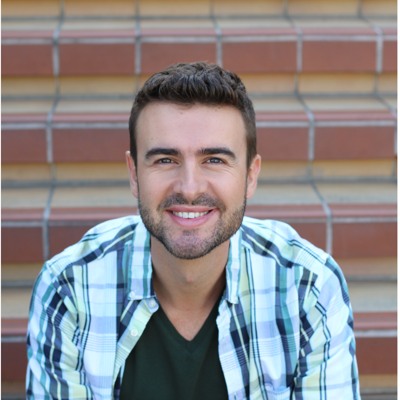
\includegraphics[width=3cm,height=3cm]{figures/persona-juan}};
        \end{scope}
        \draw[rounded corners=8pt, black!30] (0,0) rectangle (3,3);
    \end{tikzpicture}
\end{minipage}\hfill
\begin{minipage}[c]{0.72\textwidth}
    {\textbf{Juan García}} \\
    34 años - Dueño de PyME - Lanús, Buenos Aires
\end{minipage}

\begin{itemize}[leftmargin=2em]
  \item\textbf{Contexto y rol respecto al producto o sistema} \hfill \\
    Administra un local de venta de repuestos en Lanús. Necesita enviar mercadería mediana y voluminosa dos o tres veces por semana hacia clientes en diferentes partes del AMBA.
  \item\textbf{Objetivos al usar el producto} \hfill \\
    Busca una forma de obtener el servicio a un precio razonable y predecible, además de poder rastrear el envío y que el sistema maneje la logística sin que él tenga que coordinar por WhatsApp personalmente con cada uno de los clientes durante todo el día.
  \item\textbf{Frustraciones y obstáculos actuales} \hfill \\
    El flete exclusivo por cada envío es su principal costo: afecta el margen de ganancia, y trasladarlo a precios resultaría en una baja de competitividad.
  \item\textbf{Comportamientos y hábitos relevantes} \hfill \\
	Actualmente coordina los envíos a través de WhatsApp con cada cliente, lo que le demanda tiempo y genera incertidumbre sobre la llegada de los pedidos.
  \item\textbf{Cita representativa} \hfill \\
    \textit{"Necesito una forma de enviar mis productos sin tener que pagar un flete completo cada vez, y sin tener que estar pendiente de coordinar con cada cliente todo el tiempo."}
\end{itemize}

\noindent
\begin{minipage}[c]{0.24\textwidth}
    \centering
    % Fotografía del arquetipo, recortada con esquinas redondeadas.
    \begin{tikzpicture}
        \begin{scope}
            \clip[rounded corners=8pt] (0,0) rectangle (3,3);
            \node[anchor=south west, inner sep=0] at (0,0)
                {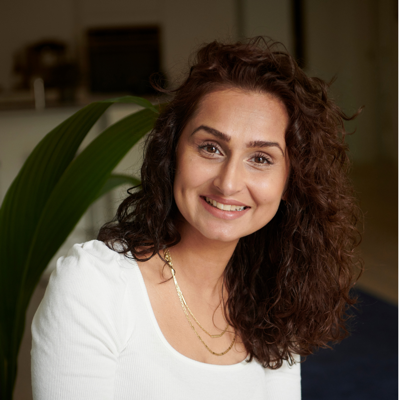
\includegraphics[width=3cm,height=3cm]{figures/persona-maria}};
        \end{scope}
        \draw[rounded corners=8pt, black!30] (0,0) rectangle (3,3);
    \end{tikzpicture}
\end{minipage}\hfill
\begin{minipage}[c]{0.72\textwidth}
    {\textbf{María Álvarez}} \\
    40 años - Trabaja en recursos humanos en una oficina en Microcentro - Caballito, CABA
\end{minipage}

\begin{itemize}[leftmargin=2em]
  \item\textbf{Contexto y rol respecto al producto o sistema} \hfill \\
    Trabaja en recursos humanos en el microcentro y hace todos los días el trayecto de Caballito a Microcentro en auto.
  \item\textbf{Objetivos al usar el producto} \hfill \\
    Busca sacarle provecho económico a un viaje que de todos modos ya realiza, sin sumar tareas que le compliquen la jornada ni la obliguen a comprometer horarios fijos.
  \item\textbf{Frustraciones y obstáculos actuales} \hfill \\
    En experiencias previas con changas le incomodó tener que estar siempre disponible y depender de responder al instante para no quedar mal evaluada. No dispone del tiempo que exige una actividad de reparto continua.
  \item\textbf{Comportamientos y hábitos relevantes} \hfill \\
	Usa el auto y por lo general viaja con el baúl vacío. \nuevo{Como valor secundario, le resulta atractivo que ese mismo trayecto evite que otro vehículo tenga que salir a la calle solo para llevar lo que ella ya puede llevar de paso.} El precio mínimo que esperaría cobrar ronda los \$3.000--\$4.000 por llevar un paquete chico.
  \item\textbf{Cita representativa} \hfill \\
    \textit{"Todos los días hago el mismo viaje al centro con el baúl vacío; si pudiera sacar algo a cambio sin complicarme la rutina, lo haría."}
\end{itemize}

\noindent
\begin{minipage}[c]{0.24\textwidth}
    \centering
    % Fotografía del arquetipo, recortada con esquinas redondeadas.
    \begin{tikzpicture}
        \begin{scope}
            \clip[rounded corners=8pt] (0,0) rectangle (3,3);
            \node[anchor=south west, inner sep=0] at (0,0)
                {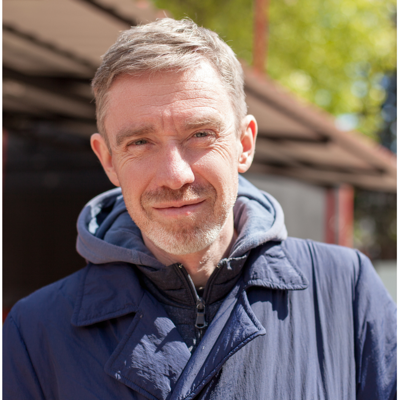
\includegraphics[width=3cm,height=3cm]{figures/persona-carlos}};
        \end{scope}
        \draw[rounded corners=8pt, black!30] (0,0) rectangle (3,3);
    \end{tikzpicture}
\end{minipage}\hfill
\begin{minipage}[c]{0.72\textwidth}
    {\textbf{Carlos Gómez}} \\
    55 años - Se dedica a hacer fletes - Quilmes, Buenos Aires
\end{minipage}

\begin{itemize}[leftmargin=2em]
  \item\textbf{Contexto y rol respecto al producto o sistema} \hfill \\
    Tiene un camión de mudanzas y actualmente consigue sus clientes a través de conocidos o por grupos de Facebook. No tiene app propia ni referencias visibles.
  \item\textbf{Objetivos al usar el producto} \hfill \\
    Quiere recibir alertas estructuradas de cargas grandes y mudanzas, con información clara del origen, destino y pago antes de confirmar.
  \item\textbf{Frustraciones y obstáculos actuales} \hfill \\
    Al depender de referencias personales, su demanda es irregular y no puede mantener un flujo constante de trabajo. Además suele encontrarse limitado a su zona de influencia, lo que restringe su capacidad de ampliar la clientela.
  \item\textbf{Comportamientos y hábitos relevantes} \hfill \\
	No le importa el desvío porque se desplaza específicamente para cada pedido a demanda del cliente.
  \item\textbf{Cita representativa} \hfill \\
    \textit{"Quisiera tener una forma más estructurada de conseguir clientes para mis fletes y al mismo tiempo generar un espacio con referencias que otros potenciales clientes puedan consultar para confiar en mi servicio."}
\end{itemize}

	{\color{nuevo}% >>> CONTENIDO NUEVO (entrega 50%) <<<
\chapter{Análisis de requerimientos}
\label{cap:requerimientos}

A partir del problema planteado, de la investigación de usuarios y de las decisiones de diseño fundamentadas en los antecedentes, se elabora el análisis funcional del sistema. Este capítulo especifica qué debe hacer DePaso (requerimientos funcionales), bajo qué restricciones de calidad debe hacerlo (requerimientos no funcionales) y cómo interactúan los distintos actores con la plataforma en sus flujos principales (casos de uso). Los requerimientos se expresan de forma independiente de la tecnología; las decisiones de implementación se abordan en el Capítulo~\ref{cap:diseno}.

% ═════════════════════════════════════════════════════════════════════════════
\section{Actores del sistema}

Se identifican cinco actores que interactúan con la plataforma:

\begin{itemize}[leftmargin=2em]
    \item \textbf{Remitente}: cliente particular, comercio o PyME que solicita un envío. Publica la carga, recibe una cotización y elige la modalidad.
    \item \textbf{Transportista}: persona que registra su trayecto habitual o su disponibilidad y transporta envíos compatibles con su recorrido. Puede operar con distintos tipos de movilidad.
    \item \textbf{PyME / organización}: entidad que agrupa a uno o varios usuarios y, opcionalmente, una flota de transportistas; programa envíos y consulta sus finanzas.
    \item \textbf{Administrador}: valida transportistas, modera la operación y ajusta los parámetros del sistema.
    \item \textbf{Sistema}: actor no humano que ejecuta procesos automáticos (clasificación de la carga, asignación por \emph{matching} y cálculo del impacto ambiental).
\end{itemize}

Un mismo usuario puede desempeñar simultáneamente los roles de remitente y transportista.

% ═════════════════════════════════════════════════════════════════════════════
\section{Requerimientos funcionales}

Los requerimientos funcionales se agrupan por subsistema. Cada uno se identifica con un código de la forma \texttt{RF-XXX-NN}, donde \texttt{XXX} indica el subsistema.

\begin{longtable}{p{2.4cm}p{11.2cm}}
    \caption{Requerimientos funcionales del sistema}
    \label{tab:rf}\\
    \toprule
    \textbf{Código} & \textbf{Descripción} \\
    \midrule
    \endfirsthead
    \multicolumn{2}{c}{\tablename\ \thetable\ -- \textit{continuación}} \\
    \toprule
    \textbf{Código} & \textbf{Descripción} \\
    \midrule
    \endhead
    \midrule
    \multicolumn{2}{r}{\textit{continúa en la página siguiente}} \\
    \endfoot
    \bottomrule
    \endlastfoot

    \multicolumn{2}{l}{\textbf{Usuarios y cuentas (RF-USR)}} \\
    RF-USR-01 & Registrar a un remitente con sus datos de contacto y credenciales. \\
    RF-USR-02 & Registrar a un transportista indicando tipo de vehículo, licencia y patente. \\
    RF-USR-03 & Autenticar a un usuario mediante sus credenciales y otorgarle una sesión. \\
    RF-USR-04 & Permitir la recuperación de la contraseña olvidada. \\
    RF-USR-05 & Consultar y editar el perfil propio. \\
    RF-USR-06 & Operar con rol dual (remitente y transportista) y alternar el modo activo. \\
    RF-USR-07 & Permitir que el administrador valide y habilite a los transportistas. \\
    \midrule
    \multicolumn{2}{l}{\textbf{Transportistas y trayectos (RF-CAR)}} \\
    RF-CAR-01 & Publicar un trayecto habitual (modalidad colaborativa) con origen, destino y ventana horaria. \\
    RF-CAR-02 & Publicar una ventana de disponibilidad (modalidad dedicada) por zona y franja horaria. \\
    RF-CAR-03 & Consultar el listado de pedidos compatibles y aceptarlos o rechazarlos. \\
    RF-CAR-04 & Actualizar el estado del envío asignado (arribo al retiro, en tránsito, entregado). \\
    RF-CAR-05 & Consultar el historial de envíos, ingresos, reputación y CO\textsubscript{2} evitado. \\
    RF-CAR-06 & Aplicar una penalización de reputación cuando el transportista cancela un envío aceptado. \\
    \midrule
    \multicolumn{2}{l}{\textbf{Envíos (RF-SHP)}} \\
    RF-SHP-01 & Crear una solicitud de envío indicando origen, destino, categoría de carga y modalidad. \\
    RF-SHP-02 & Cotizar el envío comparando la modalidad dedicada y la colaborativa. \\
    RF-SHP-03 & Permitir el ingreso manual de la categoría de carga como alternativa a la clasificación automática. \\
    RF-SHP-04 & Registrar el pago simulado del envío reteniendo la comisión de la plataforma (esquema de garantía). \\
    RF-SHP-05 & Gestionar el ciclo de vida del envío mediante una máquina de estados con transiciones válidas. \\
    RF-SHP-06 & Consultar el detalle y el historial de los envíos propios. \\
    RF-SHP-07 & Cancelar un envío, revirtiendo el pago según su estado. \\
    RF-SHP-08 & Calificar a la contraparte al finalizar el envío. \\
    \midrule
    \multicolumn{2}{l}{\textbf{Asignación inteligente (RF-MAT)}} \\
    RF-MAT-01 & Ordenar a los transportistas candidatos de un envío según un puntaje multivariable. \\
    RF-MAT-02 & Aplicar filtros duros de compatibilidad (vehículo/carga, capacidad y desvío máximo) antes del puntaje. \\
    RF-MAT-03 & Generar, para cada transportista, el listado de pedidos compatibles con su trayecto o disponibilidad. \\
    \midrule
    \multicolumn{2}{l}{\textbf{Clasificación de la carga (RF-VIS)}} \\
    RF-VIS-01 & Clasificar automáticamente la carga en una categoría volumétrica a partir de una fotografía. \\
    RF-VIS-02 & Derivar al ingreso manual cuando la confianza de la clasificación es inferior al umbral definido. \\
    RF-VIS-03 & Admitir un objeto de referencia opcional en la foto para asistir la estimación. \\
    RF-VIS-04 & Registrar cada clasificación realizada para su auditoría y posterior reentrenamiento. \\
    \midrule
    \multicolumn{2}{l}{\textbf{Seguimiento (RF-TRK)}} \\
    RF-TRK-01 & Permitir al transportista publicar su posición durante un envío activo. \\
    RF-TRK-02 & Permitir al remitente consultar la ubicación del envío en tiempo real. \\
    RF-TRK-03 & Conservar el historial de trazas de cada envío. \\
    \midrule
    \multicolumn{2}{l}{\textbf{Capacidad (RF-CAP)}} \\
    RF-CAP-01 & Gestionar la capacidad disponible de cada vehículo, reservándola y liberándola según los envíos en curso. \\
    \midrule
    \multicolumn{2}{l}{\textbf{Impacto ambiental (RF-CO2)}} \\
    RF-CO2-01 & Calcular el ahorro de CO\textsubscript{2} de un envío colaborativo frente a su escenario dedicado equivalente. \\
    RF-CO2-02 & Acumular y presentar el impacto ambiental por usuario, con equivalencias comprensibles. \\
    \midrule
    \multicolumn{2}{l}{\textbf{Organizaciones / PyMEs (RF-ORG)}} \\
    RF-ORG-01 & Gestionar organizaciones (comercio y/o flota) y sus miembros. \\
    RF-ORG-02 & Administrar la flota de transportistas vinculados a la organización (alta y baja). \\
    RF-ORG-03 & Programar envíos a nombre de la organización. \\
    RF-ORG-04 & Consultar las finanzas de la organización, distinguiendo el dinero puesto del dinero ganado. \\
    \midrule
    \multicolumn{2}{l}{\textbf{Administración (RF-ADM)}} \\
    RF-ADM-01 & Proveer un panel de monitoreo operativo de la plataforma. \\
    RF-ADM-02 & Exponer estadísticas agregadas del sistema. \\
    RF-ADM-03 & Moderar usuarios y configurar los pesos del algoritmo de asignación sin necesidad de un nuevo despliegue. \\
\end{longtable}

% ═════════════════════════════════════════════════════════════════════════════
\section{Requerimientos no funcionales}

Los requerimientos no funcionales establecen las restricciones de calidad que condicionan el diseño de la solución.

\begin{longtable}{p{2.6cm}p{11cm}}
    \caption{Requerimientos no funcionales del sistema}
    \label{tab:rnf}\\
    \toprule
    \textbf{Código} & \textbf{Descripción} \\
    \midrule
    \endfirsthead
    \multicolumn{2}{c}{\tablename\ \thetable\ -- \textit{continuación}} \\
    \toprule
    \textbf{Código} & \textbf{Descripción} \\
    \midrule
    \endhead
    \bottomrule
    \endlastfoot

    \multicolumn{2}{l}{\textbf{Seguridad (RNF-SEC)}} \\
    RNF-SEC-01 & La autenticación se basa en tokens de acceso de vigencia corta y tokens de refresco; las contraseñas se almacenan con un algoritmo de \emph{hashing} robusto. \\
    RNF-SEC-02 & Se limita la tasa de intentos de inicio de sesión para mitigar ataques de fuerza bruta. \\
    RNF-SEC-03 & Las imágenes de los paquetes se almacenan con acceso restringido mediante URLs firmadas de vigencia acotada. \\
    RNF-SEC-04 & Toda solicitud entrante se valida contra un esquema antes de procesarse. \\
    \midrule
    \multicolumn{2}{l}{\textbf{Rendimiento (RNF-PERF)}} \\
    RNF-PERF-01 & La clasificación de una imagen debe resolverse en menos de 2 segundos. \\
    RNF-PERF-02 & El seguimiento en tiempo real tolera una latencia de actualización de hasta 30 segundos. \\
    \midrule
    \multicolumn{2}{l}{\textbf{Disponibilidad (RNF-AVL)}} \\
    RNF-AVL-01 & Ante la caída de un servicio externo o la falta de conectividad, el sistema degrada con gracia y no interrumpe las funciones esenciales. \\
    \midrule
    \multicolumn{2}{l}{\textbf{Mantenibilidad (RNF-MNT)}} \\
    RNF-MNT-01 & El sistema se organiza de forma modular y por capas, con responsabilidades separadas. \\
    RNF-MNT-02 & Los módulos críticos (autenticación, envíos y asignación) mantienen una cobertura de pruebas automatizadas de al menos el 60\%. \\
    RNF-MNT-03 & La interfaz de programación (API) se documenta de forma automática. \\
    \midrule
    \multicolumn{2}{l}{\textbf{Costo y portabilidad (RNF-INF)}} \\
    RNF-INF-01 & La plataforma opera dentro de un presupuesto acotado, sobre servicios de nivel gratuito. \\
    RNF-INF-02 & El sistema es portable: puede migrar de proveedor sin modificar el código de la aplicación. \\
    \midrule
    \multicolumn{2}{l}{\textbf{Usabilidad y observabilidad (RNF-UX / RNF-OBS)}} \\
    RNF-UX-01 & La interfaz emplea español rioplatense, contraste accesible y realimentación visual de cada acción del usuario. \\
    RNF-OBS-01 & El sistema registra eventos de forma estructurada para su observabilidad. \\
    \midrule
    \multicolumn{2}{l}{\textbf{Requisitos académicos (RNF-UADE)}} \\
    RNF-UADE-01 & El modelo de clasificación de carga debe ser entrenado por el equipo (se admite aprendizaje por transferencia), sin recurrir a servicios de inferencia de terceros. \\
\end{longtable}

% ═════════════════════════════════════════════════════════════════════════════
\section{Casos de uso}

Se especifican los casos de uso correspondientes a los flujos centrales del sistema. La Figura~\ref{fig:casos-uso} resume, mediante un diagrama de casos de uso, la relación entre los actores y las funcionalidades. A continuación, cada caso indica su actor principal, precondiciones, flujo principal, flujos alternativos y postcondiciones. Los requerimientos funcionales que cada caso satisface se referencian entre paréntesis.

\begin{figure}[ht]
    \centering\color{nuevo}
    \resizebox{0.92\textwidth}{!}{%
    \begin{tikzpicture}
        % Casos de uso (columna central)
        \node[ucase] (cu1) at (0,5)    {CU-01 Solicitar envío};
        \node[ucase] (cu2) at (0,3.6)  {CU-02 Clasificar carga};
        \node[ucase] (cu3) at (0,2.2)  {CU-03 Asignar (\emph{matching})};
        \node[ucase] (cu4) at (0,0.8)  {CU-04 Publicar trayecto};
        \node[ucase] (cu5) at (0,-0.6) {CU-05 Aceptar pedido};
        \node[ucase] (cu6) at (0,-2)   {CU-06 Seguir envío};
        \node[ucase] (cu7) at (0,-3.4) {CU-07 Calificar};
        \node[ucase] (cu8) at (0,-4.8) {CU-08 Validar transportista};
        % Actores
        \node (rem) at (-6,3)    {}; \pic at (rem) {actor}; \node[font=\footnotesize, below=1.6cm of rem]{Remitente};
        \node (sis) at (-6,-1.8) {}; \pic at (sis) {actor}; \node[font=\footnotesize, below=1.6cm of sis]{Sistema};
        \node (car) at (6,0.6)   {}; \pic at (car) {actor}; \node[font=\footnotesize, below=1.6cm of car]{Transportista};
        \node (adm) at (6,-4.4)  {}; \pic at (adm) {actor}; \node[font=\footnotesize, below=1.6cm of adm]{Administrador};
        % Frontera del sistema
        \node[boundary, fit=(cu1)(cu2)(cu3)(cu4)(cu5)(cu6)(cu7)(cu8), inner sep=4mm, label=above:{\footnotesize DePaso}] {};
        % Asociaciones
        \draw (rem) -- (cu1); \draw (rem) -- (cu6); \draw (rem) -- (cu7);
        \draw (sis) -- (cu2); \draw (sis) -- (cu3);
        \draw (car) -- (cu4); \draw (car) -- (cu5); \draw (car) -- (cu6); \draw (car) -- (cu7);
        \draw (adm) -- (cu8);
    \end{tikzpicture}%
    }
    \caption{Diagrama de casos de uso del sistema}
    \label{fig:casos-uso}
\end{figure}

% ─────────────────────────────────────────────────────────────────────────────
\subsection{CU-01 --- Solicitar un envío}

\begin{itemize}[leftmargin=2em]
    \item \textbf{Actor principal}: Remitente. \quad \textbf{Actor secundario}: Sistema.
    \item \textbf{Precondiciones}: el remitente tiene una sesión activa (RF-USR-03).
    \item \textbf{Flujo principal}:
    \begin{enumerate}[leftmargin=2em]
        \item El remitente indica el origen y el destino del envío.
        \item El remitente fotografía el paquete; el sistema clasifica la carga (CU-02) o el remitente ingresa la categoría manualmente (RF-SHP-03).
        \item El sistema cotiza el envío, comparando la modalidad dedicada y la colaborativa e indicando el CO\textsubscript{2} estimado (RF-SHP-02, RF-CO2-01).
        \item El remitente elige la modalidad y confirma la solicitud (RF-SHP-01).
        \item El remitente abona el envío; el sistema retiene la comisión bajo un esquema de garantía (RF-SHP-04).
        \item El sistema crea el envío en estado \emph{pendiente} e inicia la asignación (CU-03).
    \end{enumerate}
    \item \textbf{Flujos alternativos}:
    \begin{itemize}[leftmargin=2em]
        \item[2a.] Si la confianza de la clasificación es baja, el sistema solicita la categoría manual (RF-VIS-02).
        \item[5a.] Si el pago no se completa, el envío no se crea y la solicitud queda descartada.
    \end{itemize}
    \item \textbf{Postcondiciones}: existe un envío en estado \emph{pendiente} listo para ser asignado.
\end{itemize}

% ─────────────────────────────────────────────────────────────────────────────
\subsection{CU-02 --- Clasificar la carga mediante una fotografía}

\begin{itemize}[leftmargin=2em]
    \item \textbf{Actor principal}: Sistema. \quad \textbf{Actor secundario}: Remitente.
    \item \textbf{Precondiciones}: el remitente aportó una fotografía del paquete.
    \item \textbf{Flujo principal}:
    \begin{enumerate}[leftmargin=2em]
        \item El remitente captura la imagen, opcionalmente junto a un objeto de referencia (RF-VIS-03).
        \item El sistema infiere la categoría volumétrica y su nivel de confianza (RF-VIS-01).
        \item Si la confianza supera el umbral, el sistema propone la categoría; en caso contrario, deriva al ingreso manual (RF-VIS-02).
        \item El sistema registra la clasificación para su auditoría (RF-VIS-04).
    \end{enumerate}
    \item \textbf{Flujos alternativos}:
    \begin{itemize}[leftmargin=2em]
        \item[2a.] Si el servicio de clasificación no está disponible, el sistema ofrece directamente el ingreso manual (RNF-AVL-01).
    \end{itemize}
    \item \textbf{Postcondiciones}: el envío queda asociado a una categoría de carga.
\end{itemize}

% ─────────────────────────────────────────────────────────────────────────────
\subsection{CU-03 --- Asignar un transportista mediante \emph{matching}}

\begin{itemize}[leftmargin=2em]
    \item \textbf{Actor principal}: Sistema.
    \item \textbf{Precondiciones}: existe un envío en estado \emph{pendiente}.
    \item \textbf{Flujo principal}:
    \begin{enumerate}[leftmargin=2em]
        \item El sistema aplica los filtros duros: compatibilidad de vehículo y carga, capacidad suficiente y desvío por debajo del máximo admitido (RF-MAT-02).
        \item Para cada candidato, calcula un puntaje que combina compatibilidad geográfica, desvío, carga, reputación y ventana horaria (RF-MAT-01).
        \item Ordena a los candidatos y expone el envío en el listado de los transportistas compatibles (RF-MAT-03).
        \item Cuando un transportista acepta (CU-05), el envío pasa a estado \emph{asignado} y el sistema notifica al remitente.
    \end{enumerate}
    \item \textbf{Flujos alternativos}:
    \begin{itemize}[leftmargin=2em]
        \item[1a.] Si ningún candidato supera los filtros duros, el envío permanece pendiente y se reintenta la asignación.
    \end{itemize}
    \item \textbf{Postcondiciones}: el envío queda asignado a un transportista o continúa pendiente.
\end{itemize}

% ─────────────────────────────────────────────────────────────────────────────
\subsection{CU-04 --- Publicar un trayecto habitual}

\begin{itemize}[leftmargin=2em]
    \item \textbf{Actor principal}: Transportista.
    \item \textbf{Precondiciones}: el transportista está habilitado por el administrador (RF-USR-07).
    \item \textbf{Flujo principal}:
    \begin{enumerate}[leftmargin=2em]
        \item El transportista registra el origen, el destino y la ventana horaria de su recorrido habitual (RF-CAR-01) o su ventana de disponibilidad dedicada (RF-CAR-02).
        \item El sistema valida los datos y publica el trayecto o la ventana como activos.
        \item El sistema comienza a evaluar los envíos pendientes compatibles con ese trayecto (CU-03).
    \end{enumerate}
    \item \textbf{Postcondiciones}: el transportista figura como disponible para recibir pedidos compatibles.
\end{itemize}

% ─────────────────────────────────────────────────────────────────────────────
\subsection{CU-05 --- Aceptar un pedido del listado}

\begin{itemize}[leftmargin=2em]
    \item \textbf{Actor principal}: Transportista.
    \item \textbf{Precondiciones}: el transportista tiene un trayecto o disponibilidad activos y capacidad libre (RF-CAP-01).
    \item \textbf{Flujo principal}:
    \begin{enumerate}[leftmargin=2em]
        \item El transportista consulta su listado de pedidos compatibles, con el desvío y la ganancia estimada de cada uno (RF-CAR-03).
        \item Selecciona un pedido y lo acepta.
        \item El sistema reserva la capacidad del vehículo y asigna el envío (RF-CAP-01).
        \item El transportista actualiza el estado a medida que avanza: arribo al retiro, en tránsito y entregado (RF-CAR-04, RF-SHP-05).
    \end{enumerate}
    \item \textbf{Flujos alternativos}:
    \begin{itemize}[leftmargin=2em]
        \item[2a.] Si el transportista cancela luego de aceptar, el sistema penaliza su reputación (RF-CAR-06).
    \end{itemize}
    \item \textbf{Postcondiciones}: el envío queda en curso bajo la responsabilidad del transportista.
\end{itemize}

% ─────────────────────────────────────────────────────────────────────────────
\subsection{CU-06 --- Seguir el envío en tiempo real}

\begin{itemize}[leftmargin=2em]
    \item \textbf{Actor principal}: Remitente. \quad \textbf{Actor secundario}: Transportista.
    \item \textbf{Precondiciones}: el envío está en tránsito.
    \item \textbf{Flujo principal}:
    \begin{enumerate}[leftmargin=2em]
        \item El transportista publica periódicamente su posición durante el envío (RF-TRK-01).
        \item El remitente consulta la ubicación del envío, que se actualiza de forma continua (RF-TRK-02).
        \item Al entregarse, el sistema libera el pago al transportista y persiste el CO\textsubscript{2} ahorrado (RF-SHP-05, RF-CO2-01).
    \end{enumerate}
    \item \textbf{Postcondiciones}: el envío queda entregado y su traza se conserva (RF-TRK-03).
\end{itemize}

% ─────────────────────────────────────────────────────────────────────────────
\subsection{CU-07 --- Calificar a la contraparte}

\begin{itemize}[leftmargin=2em]
    \item \textbf{Actor principal}: Remitente o Transportista.
    \item \textbf{Precondiciones}: el envío fue entregado.
    \item \textbf{Flujo principal}:
    \begin{enumerate}[leftmargin=2em]
        \item Cada parte califica a la otra con una puntuación y un comentario opcional (RF-SHP-08).
        \item El sistema actualiza la reputación acumulada de la contraparte.
    \end{enumerate}
    \item \textbf{Postcondiciones}: las reputaciones quedan actualizadas y disponibles para futuros \emph{matchings} (RF-MAT-01).
\end{itemize}

% ─────────────────────────────────────────────────────────────────────────────
\subsection{CU-08 --- Validar a un transportista}

\begin{itemize}[leftmargin=2em]
    \item \textbf{Actor principal}: Administrador.
    \item \textbf{Precondiciones}: existe un transportista registrado pendiente de validación.
    \item \textbf{Flujo principal}:
    \begin{enumerate}[leftmargin=2em]
        \item El administrador revisa los datos y la documentación del transportista (RF-USR-07).
        \item Aprueba o rechaza la solicitud (RF-ADM-03).
        \item Si se aprueba, el transportista queda habilitado para publicar trayectos y recibir pedidos.
    \end{enumerate}
    \item \textbf{Postcondiciones}: el transportista queda habilitado o rechazado.
\end{itemize}
}% <<< FIN CONTENIDO NUEVO (entrega 50%) >>>

	{\color{nuevo}% >>> CONTENIDO NUEVO (entrega 50%) <<<
\chapter{Metodología de desarrollo}
\label{cap:diseno}

Este capítulo describe cómo se construye la solución a partir del análisis de requerimientos del Capítulo~\ref{cap:requerimientos}. Se presenta la metodología de trabajo adoptada, la arquitectura de la solución y su infraestructura de red, las tecnologías seleccionadas y su justificación, el modelo de datos y, finalmente, la estrategia de validación del sistema.

% ═════════════════════════════════════════════════════════════════════════════
\section{Metodología}

El desarrollo del prototipo sigue un enfoque \textbf{iterativo e incremental}: la funcionalidad se construye en hitos sucesivos, cada uno con valor demostrable, priorizando primero la base transversal (autenticación, persistencia y ciclo de vida del envío) y avanzando luego hacia los componentes diferenciales (asignación inteligente, clasificación por visión computacional y cálculo de impacto ambiental). Este orden permite validar de forma temprana las decisiones de diseño fundamentadas en los antecedentes y ajustar el alcance según los resultados.

El trabajo se apoya en un conjunto de prácticas de ingeniería: control de versiones con Git y GitHub, empaquetado reproducible mediante contenedores, configuración externalizada por entorno, pruebas automatizadas sobre los módulos críticos e integración continua. La construcción del conjunto de datos para el clasificador se inicia en paralelo desde las primeras etapas, por ser la tarea que no puede acelerarse con código.

% ═════════════════════════════════════════════════════════════════════════════
\section{Arquitectura de la solución}

La solución adopta el patrón de \textbf{monolito modular orientado a dominio}: una única aplicación de servidor organizada en módulos autocontenidos, cada uno responsable de un dominio del negocio. Se descarta una arquitectura de microservicios porque su complejidad operativa (comunicación de red entre servicios, observabilidad distribuida y consistencia eventual) no se justifica en un prototipo de estas dimensiones; la modularización interna preserva, no obstante, límites claros que habilitarían la extracción de un servicio en el futuro si la escala lo requiriera.

La arquitectura se describe siguiendo el modelo \textbf{C4}, de mayor a menor nivel de abstracción.

\begin{itemize}[leftmargin=2em]
    \item \textbf{Contexto.} El sistema atiende a cinco tipos de actor (cliente particular, transportista, PyME fletera, PyME comercio y administrador) a través de dos frentes —una aplicación móvil para clientes y transportistas y un panel web para PyMEs y administración— sobre un único backend. Sus dependencias externas son mínimas y reemplazables: un servicio de ruteo (con alternativa de cálculo propia), un servicio de mapas y geocodificación, y la persistencia de datos e imágenes.
    \item \textbf{Contenedores.} Las unidades desplegables por separado son: la aplicación móvil, el panel web, la API REST, la base de datos y el almacenamiento de objetos. Las aplicaciones cliente se comunican con la API sobre HTTPS con autenticación por token; la API concentra toda la lógica de negocio y el acceso a datos.
    \item \textbf{Componentes.} Dentro de la API, cada módulo de dominio respeta una separación estricta en cuatro capas —enrutamiento (HTTP y validación), servicio (lógica de negocio), repositorio (acceso a datos) y esquemas—, con una regla de dependencia unidireccional. Los módulos implementados abarcan autenticación, usuarios, transportistas, envíos, trayectos, asignación, visión, seguimiento, capacidad, impacto ambiental, organizaciones y administración.
\end{itemize}

La Figura~\ref{fig:c4-contexto} representa el nivel de contexto: el sistema como una caja negra, sus usuarios y sus dependencias externas.

\begin{figure}[ht]
    \centering\color{nuevo}
    \begin{tikzpicture}
        \node[c4system] (S) at (0,0) {\textbf{DePaso}\\ Logística urbana\\ colaborativa};
        % Actores
        \node[c4person] (cli) at (-5.6,2.7)  {Cliente\\ particular};
        \node[c4person] (tra) at (-5.6,0.9)  {Transportista};
        \node[c4person] (pf)  at (-5.6,-0.9) {PyME fletera};
        \node[c4person] (pc)  at (-5.6,-2.7) {PyME comercio};
        \node[c4person] (adm) at (0,-3.4)    {Administrador};
        % Dependencias externas
        \node[c4ext] (osrm) at (5.6,1.8)  {Servicio de\\ ruteo};
        \node[c4ext] (maps) at (5.6,0)    {Mapas /\\ geocodificación};
        \node[c4db]  (db)   at (5.6,-2.1) {Base de datos\\ + almacenamiento};
        % Actores -> sistema
        \draw[c4arrow] (cli) -- (S);
        \draw[c4arrow] (tra) -- (S);
        \draw[c4arrow] (pf)  -- (S);
        \draw[c4arrow] (pc)  -- (S);
        \draw[c4arrow] (adm) -- (S);
        % Sistema -> externos
        \draw[c4arrow] (S) -- (osrm) node[c4lbl] {distancias};
        \draw[c4arrow] (S) -- (maps) node[c4lbl] {direcciones};
        \draw[c4arrow] (S) -- (db)   node[c4lbl] {persistencia};
    \end{tikzpicture}
    \caption{Diagrama de contexto del sistema (C4, nivel 1)}
    \label{fig:c4-contexto}
\end{figure}

La Figura~\ref{fig:c4-contenedores} desglosa el sistema en sus contenedores desplegables.

\begin{figure}[ht]
    \centering\color{nuevo}
    \begin{tikzpicture}
        \node[c4container] (app) at (-2.9,3.2) {App móvil\\ (clientes y\\ transportistas)};
        \node[c4container] (web) at (2.9,3.2)  {Panel web\\ (PyMEs y\\ administración)};
        \node[c4container, minimum width=3.4cm] (api) at (0,0.6) {\textbf{API REST}\\ lógica de negocio};
        \node[c4ext] (osrm) at (5,0.6)     {Servicio de\\ ruteo};
        \node[c4db]  (db)   at (-2.9,-2.6) {Base de\\ datos};
        \node[c4db]  (st)   at (0.2,-2.6)  {Almacenamiento\\ de objetos};
        \node[c4ext] (ml)   at (3.2,-2.6)  {Modelo de\\ IA (.\,keras)};
        \draw[c4arrow] (app) -- (api) node[c4lbl] {HTTPS + \emph{token}};
        \draw[c4arrow] (web) -- (api) node[c4lbl] {HTTPS + \emph{token}};
        \draw[c4arrow] (api) -- (db);
        \draw[c4arrow] (api) -- (st);
        \draw[c4arrow, dashed] (api) -- (ml)   node[c4lbl] {carga inicial};
        \draw[c4arrow, dashed] (api) -- (osrm) node[c4lbl] {o alternativa};
    \end{tikzpicture}
    \caption{Diagrama de contenedores (C4, nivel 2)}
    \label{fig:c4-contenedores}
\end{figure}

Internamente, cada contenedor de la API se organiza en módulos de dominio con cuatro capas, como muestra la Figura~\ref{fig:c4-componentes}.

\begin{figure}[ht]
    \centering\color{nuevo}
    \begin{tikzpicture}
        \node[c4container] (l1) at (0,2.4)  {Enrutamiento\\ (HTTP, validación)};
        \node[c4container] (l2) at (0,0.8)  {Servicios\\ (lógica de negocio)};
        \node[c4container] (l3) at (0,-0.8) {Repositorios\\ (acceso a datos)};
        \draw[c4arrow] (l1) -- (l2);
        \draw[c4arrow] (l2) -- (l3);
        \node[c4ext, text width=3cm] (mods) at (-4.3,0.8) {Módulos de dominio: auth, usuarios, transportistas, envíos, \emph{matching}, trayectos, seguimiento, visión, CO\textsubscript{2}, organizaciones, administración};
        \node[c4ext, text width=2.6cm] (core) at (4.3,2.2) {\emph{core}: configuración, seguridad, base de datos};
        \node[c4ext, text width=2.6cm] (shr)  at (4.3,-0.6) {\emph{shared}: geo, ruteo, enums, repositorio base};
        \node[c4db] (db) at (0,-2.7) {Base de datos};
        \draw[c4arrow] (l3) -- (db);
        \draw[c4arrow, dashed] (mods) -- (l1);
        \draw[c4arrow, dashed] (l1) -- (core);
        \draw[c4arrow, dashed] (l2) -- (shr);
        \node[boundary, fit=(l1)(l2)(l3), inner sep=5mm] {};
    \end{tikzpicture}
    \caption{Componentes del backend: módulos de dominio en cuatro capas (C4, nivel 3)}
    \label{fig:c4-componentes}
\end{figure}

Finalmente, la Figura~\ref{fig:secuencia} integra los tres pilares del proyecto —clasificación, asignación y cálculo de impacto— en el flujo de un envío colaborativo de punta a punta.

\begin{figure}[ht]
    \centering\color{nuevo}
    \resizebox{\textwidth}{!}{%
    \begin{tikzpicture}[
        msg/.style={-{Stealth[length=2mm]}, font=\scriptsize},
        ret/.style={-{Stealth[length=2mm]}, dashed, font=\scriptsize},
        part/.style={draw, fill=RoyalBlue!12, minimum height=0.8cm, font=\footnotesize, align=center},
    ]
        \node[part] (C) at (0,0)    {Cliente};
        \node[part] (A) at (3.2,0)  {App móvil};
        \node[part] (P) at (6.8,0)  {API};
        \node[part] (D) at (10.2,0) {Base de datos};
        \node[part] (R) at (13.2,0) {Cadete};
        \foreach \n in {C,A,P,D,R} { \draw[dashed, black!45] (\n.south) -- ($(\n.south)+(0,-12.8)$); }
        \draw[msg] (C|-0,-1.2)  -- (A|-0,-1.2)  node[midway,above]{fotografía el paquete};
        \draw[msg] (A|-0,-2.2)  -- (P|-0,-2.2)  node[midway,above]{clasificar carga};
        \draw[ret] (P|-0,-3.2)  -- (A|-0,-3.2)  node[midway,above]{categoría + confianza};
        \draw[msg] (A|-0,-4.2)  -- (P|-0,-4.2)  node[midway,above]{cotizar (dedicado / colaborativo + CO\textsubscript{2})};
        \draw[msg] (A|-0,-5.2)  -- (P|-0,-5.2)  node[midway,above]{crear y pagar el envío};
        \draw[msg] (P|-0,-6.2)  -- (D|-0,-6.2)  node[midway,above]{registrar envío y pago (garantía)};
        \draw[msg] (R|-0,-7.2)  -- (P|-0,-7.2)  node[midway,above]{consultar pedidos compatibles};
        \draw[msg] (R|-0,-8.2)  -- (P|-0,-8.2)  node[midway,above]{aceptar el envío};
        \draw[ret] (P|-0,-9.2)  -- (C|-0,-9.2)  node[midway,above]{notificar asignación};
        \draw[msg] (R|-0,-10.2) -- (P|-0,-10.2) node[midway,above]{actualizar estado (retiro $\to$ tránsito $\to$ entregado)};
        \draw[msg] (P|-0,-11.2) -- (D|-0,-11.2) node[midway,above]{liberar pago y persistir CO\textsubscript{2}};
        \draw[msg] (C|-0,-12.4) -- (P|-0,-12.4) node[midway,above]{calificar};
    \end{tikzpicture}%
    }
    \caption{Diagrama de secuencia: envío colaborativo de punta a punta}
    \label{fig:secuencia}
\end{figure}

% ─────────────────────────────────────────────────────────────────────────────
\subsection{Arquitectura de red e infraestructura}

La topología de despliegue se diseña bajo la restricción de presupuesto acotado (RNF-INF-01), sobre servicios gestionados de nivel gratuito. Las aplicaciones cliente —la app móvil, distribuida como paquete instalable, y el panel web, publicado como sitio estático— se comunican con la API REST exclusivamente sobre HTTPS, adjuntando el token de sesión en cada solicitud. La API se ejecuta dentro de un contenedor sobre una plataforma como servicio (PaaS) y se conecta a una base de datos PostgreSQL gestionada y a un almacenamiento de objetos para las imágenes de los paquetes. El servicio de ruteo es opcional: ante su ausencia, el sistema degrada de forma automática a una estimación de distancias propia (RNF-AVL-01).

El flujo de integración y despliegue continuo se apoya en el control de versiones: cada publicación de cambios dispara el despliegue automático del backend y del panel web, mientras que el paquete de la aplicación móvil se genera mediante el servicio de compilación correspondiente. Esta elección mantiene la portabilidad del sistema (RNF-INF-02): migrar de proveedor implica cambiar dónde se ejecuta el mismo contenedor, no el código de la aplicación.

La Figura~\ref{fig:despliegue} sintetiza la topología de despliegue y el flujo de integración y despliegue continuo.

\begin{figure}[ht]
    \centering\color{nuevo}
    \begin{tikzpicture}
        \node[c4ext, text width=2.4cm] (dev) at (-6,1.6)  {Desarrollo local (contenedores)};
        \node[c4ext] (gh) at (-6,-1) {Repositorio\\ (GitHub)};
        \node[c4container] (ren) at (1.2,1.7) {API\\ (contenedor)};
        \node[c4container] (ver) at (4.4,1.7) {Panel web\\ (sitio estático)};
        \node[c4db] (sup) at (2.7,-0.6) {Base de datos\\ + almacenamiento};
        \node[c4ext] (eas) at (-2.6,-3.5) {Servicio de\\ compilación};
        \node[c4ext] (and) at (1.2,-3.5)  {Teléfono\\ (paquete móvil)};
        \draw[c4arrow] (dev) -- (gh) node[c4lbl] {publica};
        \draw[c4arrow] (gh) -- (ren) node[c4lbl, pos=0.68] {despliegue};
        \draw[c4arrow] (gh) -- (ver) node[c4lbl, pos=0.48] {despliegue};
        \draw[c4arrow] (gh) -- (eas) node[c4lbl] {compila};
        \draw[c4arrow] (eas) -- (and) node[c4lbl] {paquete};
        \draw[c4arrow] (ren) -- (sup);
        \draw[c4arrow, dashed] (ver) -- (ren) node[c4lbl] {API};
        \draw[c4arrow] (and) -- (ren) node[c4lbl, pos=0.55] {HTTPS};
        \node[boundary, fit=(ren)(ver)(sup), inner sep=5mm, label=above:{\footnotesize Nube --- nivel gratuito}] {};
    \end{tikzpicture}
    \caption{Diagrama de despliegue: topología de infraestructura e integración continua}
    \label{fig:despliegue}
\end{figure}

% ═════════════════════════════════════════════════════════════════════════════
\section{Tecnologías utilizadas}

La selección de tecnologías responde a los requerimientos no funcionales y a las decisiones de diseño fundamentadas en los antecedentes. La Tabla~\ref{tab:stack} resume el \emph{stack} adoptado y su justificación.

\begin{longtable}{p{3.1cm}p{4.4cm}p{6cm}}
    \caption{Tecnologías seleccionadas y su justificación}
    \label{tab:stack}\\
    \toprule
    \textbf{Capa} & \textbf{Tecnología} & \textbf{Justificación} \\
    \midrule
    \endfirsthead
    \multicolumn{3}{c}{\tablename\ \thetable\ -- \textit{continuación}} \\
    \toprule
    \textbf{Capa} & \textbf{Tecnología} & \textbf{Justificación} \\
    \midrule
    \endhead
    \bottomrule
    \endlastfoot

    Backend & Python con FastAPI (asíncrono) & Concurrencia nativa para operaciones de entrada/salida, documentación de API autogenerada (RNF-MNT-03) y validación de datos integrada (RNF-SEC-04). \\
    Persistencia & PostgreSQL con extensión geoespacial & Soporte nativo de tipos y consultas geográficas, necesario para la compatibilidad geográfica del \emph{matching}; disponible en nivel gratuito (RNF-INF-01). \\
    Acceso a datos & Mapeo objeto-relacional asíncrono & Aísla la lógica de negocio del motor de base de datos y facilita las pruebas (patrón repositorio, RNF-MNT-01). \\
    Autenticación & Tokens de acceso y refresco con \emph{hashing} de contraseñas & Sesiones seguras sin estado y almacenamiento resistente de credenciales (RNF-SEC-01). \\
    Ruteo y distancias & Servicio de ruteo por calles con alternativa propia & Cálculo de desvío real y de distancias para el \emph{matching} y el CO\textsubscript{2}, con degradación automática (RNF-AVL-01). \\
    Modelo de IA & Red convolucional preentrenada con aprendizaje por transferencia & Clasificación volumétrica de la carga con un conjunto de datos acotado, entrenada por el equipo (RNF-UADE-01). \\
    Aplicación móvil & React Native con Expo & Desarrollo multiplataforma desde una única base de código, con distribución de paquetes instalables. \\
    Panel web & Aplicación de página única & Interfaz de escritorio para PyMEs y administración (tablas densas y gráficos) que consume la misma API. \\
    Almacenamiento de imágenes & Almacenamiento de objetos con URLs firmadas & Acceso restringido y temporal a las fotos de los paquetes (RNF-SEC-03). \\
    Infraestructura & Contenedores sobre plataforma como servicio & Portabilidad (RNF-INF-02) y despliegue sin administración de servidores, en nivel gratuito (RNF-INF-01). \\
    Observabilidad & Registro estructurado de eventos & Trazabilidad de la operación (RNF-OBS-01). \\
    Pruebas e integración & Marco de pruebas automatizadas e integración continua & Cobertura de los módulos críticos y verificación en cada cambio (RNF-MNT-02). \\
\end{longtable}

En el núcleo del componente de inteligencia artificial se emplea aprendizaje por transferencia sobre una red convolucional preentrenada: en lugar de entrenar un modelo desde cero —inviable con el volumen de datos disponible—, se reutiliza una arquitectura con capacidades visuales genéricas y se la adapta al dominio del problema, cumpliendo el requisito de un modelo entrenado por el equipo (RNF-UADE-01) y la restricción de inferencia local sin servicios de terceros.

% ═════════════════════════════════════════════════════════════════════════════
\section{Modelo de datos}

El modelo de datos se organiza en torno a las entidades del dominio. La Tabla~\ref{tab:entidades} describe las principales; las relaciones más relevantes vinculan a un usuario con su perfil de transportista, a este con sus trayectos publicados, y a cada envío con su cliente, su transportista asignado, su clasificación de carga y sus eventos de estado.

\begin{longtable}{p{3.2cm}p{10.4cm}}
    \caption{Entidades principales del modelo de datos}
    \label{tab:entidades}\\
    \toprule
    \textbf{Entidad} & \textbf{Descripción} \\
    \midrule
    \endfirsthead
    \multicolumn{2}{c}{\tablename\ \thetable\ -- \textit{continuación}} \\
    \toprule
    \textbf{Entidad} & \textbf{Descripción} \\
    \midrule
    \endhead
    \bottomrule
    \endlastfoot

    Usuario & Datos de contacto y credenciales; tipo (particular o comercial) y roles (cliente, transportista). \\
    Transportista & Perfil asociado a un usuario: tipo de vehículo, licencia, patente, estado de validación, reputación y capacidad. \\
    Trayecto & Recorrido habitual (colaborativo) o ventana de disponibilidad (dedicada), con origen, destino, geometría y ventana horaria. \\
    Envío & Solicitud de transporte: origen, destino, modalidad, categoría de carga, estado, estado de pago, precio, ventana horaria y CO\textsubscript{2} ahorrado. \\
    Evento de envío & Registro de auditoría de cada transición de estado del envío, con marca temporal y ubicación. \\
    Clasificación & Resultado de la clasificación de la carga: imagen, categoría predicha, confianza, aceptación y categoría manual eventual. \\
    Traza GPS & Posiciones publicadas por el transportista durante un envío, para el seguimiento en tiempo real. \\
    Calificación & Puntuación y comentario asociados a un envío entregado. \\
    Pesos de asignación & Parámetros configurables del algoritmo de \emph{matching}, editables por administración. \\
    Organización & PyME (comercio y/o flota) con sus miembros, su flota de transportistas vinculados y sus envíos. \\
    \bottomrule
\end{longtable}

Los atributos geográficos (orígenes, destinos, geometrías de trayecto y trazas) se modelan con tipos espaciales e índices específicos, que sustentan las consultas de proximidad del \emph{matching}. El ciclo de vida del envío se gobierna mediante una máquina de estados (pendiente $\rightarrow$ asignado $\rightarrow$ retirado $\rightarrow$ en tránsito $\rightarrow$ entregado, con transición a cancelado), donde cada cambio válido se registra como un evento de auditoría (RF-SHP-05).

La Figura~\ref{fig:der} presenta el diagrama entidad-relación con las entidades principales y sus cardinalidades.

\begin{figure}[ht]
    \centering\color{nuevo}
    \resizebox{0.96\textwidth}{!}{%
    \begin{tikzpicture}[
        rel/.style={-, thick, black!70},
        card/.style={font=\scriptsize, fill=white, inner sep=1pt},
    ]
        \node[entity, text width=2.5cm] (usr)  at (-5.6,2.6)  {\textbf{Usuario}\nodepart{second}email, tipo, roles};
        \node[entity, text width=2.6cm] (tra)  at (-5.6,-1)   {\textbf{Transportista}\nodepart{second}vehículo, patente, estado, reputación};
        \node[entity, text width=2.6cm] (tray) at (-5.6,-4.7) {\textbf{Trayecto}\nodepart{second}tipo, origen, destino, ventana};
        \node[entity, text width=3cm]   (env)  at (0,-1)      {\textbf{Envío}\nodepart{second}origen, destino, modalidad, categoría, estado, precio, CO\textsubscript{2}};
        \node[entity, text width=2.5cm] (cla)  at (0,2.7)     {\textbf{Clasificación}\nodepart{second}categoría, confianza};
        \node[entity, text width=2.4cm] (evt)  at (5.2,2.7)   {\textbf{Evento de envío}\nodepart{second}estado, marca temporal};
        \node[entity, text width=2.4cm] (cal)  at (5.2,-1)    {\textbf{Calificación}\nodepart{second}estrellas, comentario};
        \node[entity, text width=2.4cm] (gps)  at (5.2,-4.7)  {\textbf{Traza GPS}\nodepart{second}posición, marca temporal};
        \node[entity, text width=2.5cm] (org)  at (0,-5)      {\textbf{Organización}\nodepart{second}nombre, CUIT, tipo};
        \draw[rel] (usr)  -- (tra)  node[card,pos=0.12]{1} node[card,pos=0.9]{0..1};
        \draw[rel] (tra)  -- (tray) node[card,pos=0.12]{1} node[card,pos=0.9]{N};
        \draw[rel] (usr)  -- (env)  node[card,pos=0.12]{1} node[card,pos=0.9]{N};
        \draw[rel] (tra)  -- (env)  node[card,pos=0.12]{1} node[card,pos=0.9]{N};
        \draw[rel] (env)  -- (cla)  node[card,pos=0.12]{1} node[card,pos=0.9]{0..1};
        \draw[rel] (env)  -- (evt)  node[card,pos=0.12]{1} node[card,pos=0.9]{N};
        \draw[rel] (env)  -- (cal)  node[card,pos=0.12]{1} node[card,pos=0.9]{N};
        \draw[rel] (env)  -- (gps)  node[card,pos=0.12]{1} node[card,pos=0.9]{N};
        \draw[rel] (org)  -- (env)  node[card,pos=0.12]{1} node[card,pos=0.9]{N};
        \draw[rel] (org)  -- (tra)  node[card,pos=0.12]{1} node[card,pos=0.9]{N};
    \end{tikzpicture}%
    }
    \caption{Diagrama entidad-relación del modelo de datos}
    \label{fig:der}
\end{figure}

% ═════════════════════════════════════════════════════════════════════════════
\section{Validación del sistema}

La validación combina pruebas automatizadas del software y evaluación cuantitativa del modelo de inteligencia artificial.

En el backend, los módulos críticos —autenticación, envíos y asignación— se cubren con pruebas automatizadas, con el objetivo de una cobertura de al menos el 60\% (RNF-MNT-02). El diseño favorece esta verificación: los cálculos centrales del \emph{matching} y del CO\textsubscript{2} se implementan como funciones puras y determinísticas, lo que permite comprobar de forma directa la tabla de compatibilidad vehículo-carga, los filtros duros (descarte de la modalidad colaborativa para cargas voluminosas, de la movilidad a pie o en bicicleta en trayectos largos y de los desvíos por encima del máximo admitido), el ordenamiento por proximidad y el cálculo del ahorro de emisiones con coordenadas reales del AMBA.

El modelo de clasificación de carga se evalúa exclusivamente sobre el conjunto de prueba, reservado hasta la instancia final. Se reportan la exactitud global, la precisión, la exhaustividad y la medida F por categoría, y la matriz de confusión, prestando atención a las confusiones entre categorías adyacentes. Complementariamente, se realiza un análisis de sesgos que agrupa el conjunto de prueba según las condiciones de captura —iluminación, ángulo y fondo— y según la presencia de un objeto de referencia, calculando la exactitud por grupo para detectar y documentar las condiciones en las que el desempeño se degrada (RNF-UADE-01). Este análisis alimenta tanto las mitigaciones del modelo como las recomendaciones de uso en la interfaz.
}% <<< FIN CONTENIDO NUEVO (entrega 50%) >>>

	\chapter{Conclusión parcial}\label{conclusions}
{\color{nuevo}% >>> CONTENIDO ACTUALIZADO (entrega 50%) <<<

\section{Resumen de aportes al 50\%}

El presente avance consolida los fundamentos conceptuales y empíricos del proyecto DePaso y progresa hacia el análisis funcional y el diseño de la solución. El Capítulo~2 construyó un marco teórico organizado en cinco subtemas vinculados a decisiones concretas de diseño: el modelo de crowdsourced delivery y su contexto en la logística de última milla, la lógica de flotas híbridas y el problema del desvío, la taxonomía de perfiles de conductores (gig-workers y conductores ocasionales), el diseño de mercados de matching y asignación, y la visión computacional y el aprendizaje por transferencia, complementados por la declaración del plan de datos del clasificador (procedencia, volumen y tratamiento del conjunto de entrenamiento). El análisis del estado del arte, con estrategia de búsqueda documentada, matriz de siete antecedentes y análisis de tendencias emergentes, confirmó que ningún actor del mercado argentino combina los cinco atributos diferenciadores de DePaso: modelo híbrido dedicado--colaborativo, clasificador de carga por IA propio, control del desvío como variable ambiental explícita, cálculo de CO\textsubscript{2} ahorrado por envío y adaptación específica al contexto del AMBA. Este relevamiento se complementó con un análisis competitivo mediante las cinco fuerzas de Porter y una matriz FODA, que ubican a la plataforma en un segmento no atendido y sustentan su viabilidad estratégica.

El Capítulo~3 presentó los resultados de la encuesta, con 145 respuestas completas, que validan tres supuestos centrales del proyecto: (1)~disposición suficiente al modelo colaborativo (69,8\% del lado remitente); (2)~masa crítica potencial de transportistas (84,5\% de quienes respondieron el bloque, con disposición condicional o definitiva); y (3)~superposición entre la disposición a pagar del remitente y la compensación mínima del transportista, con margen operativo positivo para la plataforma.

El Capítulo~4 formalizó el análisis de requerimientos: se especificaron los requerimientos funcionales y no funcionales del sistema y se modelaron los casos de uso de los flujos centrales, estableciendo con precisión qué debe hacer la plataforma y bajo qué restricciones de calidad.

El Capítulo~5 definió la metodología de desarrollo y el diseño de la solución: una arquitectura de monolito modular documentada con el modelo C4, el stack tecnológico seleccionado y justificado, el modelo de datos y la estrategia de validación del sistema. De este modo, los cinco atributos diferenciadores dejan de ser una propuesta conceptual para materializarse en un diseño concreto y verificable.

\section{Trabajo futuro}

Las actividades previstas para completar el proyecto hacia diciembre de 2026 incluyen:

\begin{itemize}[leftmargin=2em]
    \item Validación y refinamiento de las user personas preliminares a partir de la ampliación de la muestra de la encuesta, que permanece abierta.
    \item Entrenamiento y evaluación del clasificador de carga por visión computacional, incluido el análisis de sesgos (agosto--noviembre).
    \item Continuación del desarrollo del prototipo funcional (backend, frontend y algoritmo de matching) sobre la arquitectura definida (hasta octubre).
    \item Integración, pruebas de sistema y validación con usuarios reales (octubre--noviembre).
    \item Redacción del informe final y preparación de la defensa (noviembre--diciembre).
\end{itemize}
}% <<< FIN CONTENIDO ACTUALIZADO (entrega 50%) >>>


	\printbibliography[heading=bibintoc]

	\appendix
	\input{chapters/appendix/annex}
	\newpage
	\listoffigures
	\newpage
	\listoftables
\end{document}
